\chapter{Implementation}
\label{ch:implementation}

\section{Overview}

This chapter outlines the proposed implementation of a receiver design, for wide-band jammer scenarios and low-mobility situations.  An adaptive signal processing software solution for mitigating the effects of both intentional and unintentional jamming (including wide-band jamming) through a combination of three techniques.  These include: antenna subset selection, spectral subtraction, and signal separation, which work in conjunction with one another to extract specific transmissions from a mixture of intercepted wireless signals. The goal of the proposed solution, originally called BLInd Spectrum Separation (BLISS), is to enable reliable, high throughput, and robust end-to-end wireless communications, especially high capacity multimedia (voice, data, imagery) transmissions. This was later rename to AS\textsuperscript{6}.  In particular, the focus of the proposed work is the so-called ``disadvantaged user''.  These users are generally considered limited in transmission and processing power such as small-deck combatants, submarines, unmanned air vehicles (UAVs), dispersed ground units in urban and radio frequency (RF) challenged environments \cite{midterm_report}.  The previous research is also discussed for each section and implementation consideration are examined from this work.\\

\begin{figure}
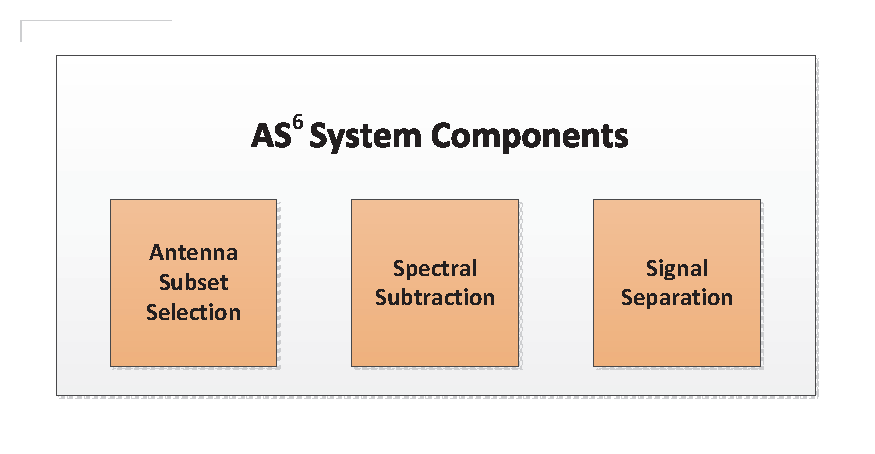
\includegraphics[width=0.75\textwidth]{as6_blocks.eps}
\caption{The AS\textsuperscript{6} system is made up of three primary blocks: antenna subset selection, spectral subtraction, and signal separation.  These combine to provide reliable signal reception in low-mobility spectral environments}
\end{figure}

The AS\textsuperscript{6} solution integrates three well-known adaptive signal processing algorithms found in the open literature: antenna subset selection \cite{antss}, spectral subtraction \cite{boll}, and signal separation \cite{AMUSE}. Each of these algorithms is employed within the AS\textsuperscript{6} framework in order to enable the process of extracting individual transmissions intercepted from several mixtures of wireless signals. Although signal separation can readily extract transmissions under ideal conditions, the AS\textsuperscript{6} system is aimed at harsh spectral environments consisting of many users and in some cases jamming devices. Therefore AS\textsuperscript{6} will not provide adequate signal separation for robust throughput.  Hence, the other two algorithms, spectral subtractions and antenna subset selection, will aid in this effort.\\

In previous sections it has been understood that current anti-jamming techniques cannot compensate in deterministic wide-band jamming scenarios.  These scenarios must be throughly understood before a practical solution can be provided.  For this thesis, the worst case scenario will be considered for the jamming device.  Since wide-band jamming devices are difficult to build, a band limited interferer was chosen instead to implement while placing restrictions on the communicating transceivers themselves.  For simplification a narrow-band jammer will be considered as an adversary, and the communicating devices cannot frequency hop thus remaining on the same frequency as the jammer.  The jammer has an identical modulation scheme as the friendly radios and the constellation is in phase.  Finally, the jammer is assumed at a similar distance and transmit power as the friendly communicating devices.  Under these conditions, the jammer is completely non-orthogonal and historically impossible to remove.\\

This chapter is broken down into several sections which include a system level overview, the hardware and software chosen, signal removal evaluation, the superimposed equalizer design, and the antenna subset selection work.  Each of the systems that makeup AS\textsuperscript{6} have different purposes and goals allowing them to tackle different problems that occur.  It is important to note that these systems are at differing stages of development due to the limited time and initial development put into these blocks.\\ 

\section{System}

To provide a more straight-forward explanation of the AS\textsuperscript{6} system, it is appropriate to provided a system level overview.  The system's original purpose was to remove the effects of narrow and wide-band jamming.  It accomplishes this goal through a series of processing blocks and a selection block.  These blocks include: the antenna subset selection (AntSS) block, spectral subtraction block, and finally the signal separation block.  The figure below shows the interconnections between these blocks and certain modification were made from the original design of the system due to practical constraints.  These changes will be brought fourth as the blocks themselves are discussed in detail. Since collaborating research group is responsible to the AntSS block, it will not be throughly discussed by this thesis, but its fundamental purpose will be examined.\\

\begin{figure}[!ht]\label{bliss_system}
\hspace{0.2in}
\includegraphics[width=0.75\textwidth]{bliss_system.eps}
\caption{Overview of the original BLISS system as present in the proposal document \cite{onr_original}, outlines three basic blocks: antenna subset selection, spectral subtraction, and blind source separation.}
\end{figure}

The first step in the AS\textsuperscript{6} system is to pass through the AntSS block.  Physically this block is equipped with many antenna in groups of 4.  As the block title portrays a subset of these antennas will be selected and they will be passed on to the next block.  In particular, a \(2^{M}-to-2^{N}\) down selection from an array of receive antennas to a set of BLISS receiver inputs is performed. Each individual AntSS board provides 4-to-2 antenna down selection through a set of RF switches.  The goal of AntSS is to provide spatial separation through an array of antennas maximizing the SNR of the wanted signal.  It is important to note that the antenna spacing must be adequate to provide enough separation or independence, depending on the operating frequencies or wavelength of the signals themselves.  Once the appropriate antennas are selected two signals are to the spectral subtraction block.\\

The Spectral Subtraction block is next, which is used to removal known unwanted signal from the spectrum so the source separation block and work properly.  The original design of the spectral subtraction block is to use an existing audio technique of removing noise or signals in the frequency domain through a subtraction and smoothing technique.  This technique was discussed previously in the background section, therefore its historical literature will not be examined further.  To enable the removal of unwanted signals, the Spectral Subtraction block maintains a database of known power spectral densities (PSD) of common modulation schemes.  A recognition system would be implemented to automatic identification of the interfering signal and the block would simply subtract it out, through its already known estimate from its database.  Next, the subtracted signal is passed to the Signal Separation System, where the signal is unmixed.\\

The Signal Separation block separates signals when only their mixtures are observed.  The operation is called blind, since the signal sources and mixing procedure are unknown to the receiver.  Under several conditions, this constraint cannot be completely upheld.  This is true because the solutions needed to solve such an event become generally intractable.  An initial approach in this project was to use a technique called AMUSE (Algorithm for Multiple Unknown Signals Extraction) \cite{AMUSE}.  AMUSE works by first collecting an estimate of the covariance matrix of the received signal \(R_{y}=E[yy^\top]\). Then computing the singular value decomposition of that covariance matrix, and estimating the number of sources, noise variance \(\sigma\) and singular values \(\psi_{1},\psi_{2},...,\psi_{N},\).  Next a data transform is done \(z=Cy\), where \(C = diag(1/\psi(1),1/\psi(2),1/\psi(3),...,1/\psi(N),)\).  Then an offset \(\tau\) is selected and \(R_{z}=E[z(t)z(t-\tau)^\top]\) is estimated.  From this estimate an eigenvalue decomposition is done on \(\frac{R_{z}(\tau)+R_{z}(\tau)^\top}{2}\) and the singular values are collected in \(\Sigma\).  Finally an estimate of the signal sources can be computed \(\^s=\Sigma C y\).  

It is important to note that for simplicity the mixing matrix for the original proposed solution involving AMUSE is generally constructed as a linear time invariant (LTI) system.  There is some activity occurring with nonlinear mixing, but that was considered outside of the scope of this problem.\\

\section{Hardware and Software Platforms}

Before any implementation was considered a platform needed to be chosen for the end result.  This selection provided the work flow-path for the implementation, eliminating many options.  As discussed in previous chapters, the end result wants to leverage the power of Software-Defined radios (SDR).  The hardware platform chosen was the USRP2 designed and built by Ettus Research \cite{USRP2Stats}.  These radios are readily available in the Wireless Innovation Laboratory and since the number of radios required for the design was still unknown, it was an obvious choice.  There are several software packages that support the USRP2 hardware and several will be examined in this chapter.\\

The USRP2's or Universal Software Radio Peripherals (Version 2) is a comparatively inexpensive hardware platform for software radio, and is commonly used by research labs, universities, and hobbyists \cite{wired}.  The USRP2 connects directly to a host computer through a Gigabit Ethernet link, which relays baseband sample that have been receiver or to be translated.   The motherboard provides the following subsystems: clock generation and synchronization, FPGA, ADCs, DACs, host processor interface, and power regulation. Several of these component are seen in the image in Figure \ref{usrp2_full_hardware}.  These are the basic components that are required for baseband processing of signals. A modular front-end, called a daughtercard, is used for analog operations such as up and down conversion, filtering, and other signal conditioning. By replacing this RF daughtercard many different frequency ranges can be examined.\\

\begin{figure}\label{usrp2_full_hardware}
\centering
\includegraphics[scale=0.1]{usrp2_overview3.eps}
\caption{Full USRP2 hardware with daughtercard}
\end{figure}

%\begin{figure}\label{usrp2_mainboard}
%\centering
%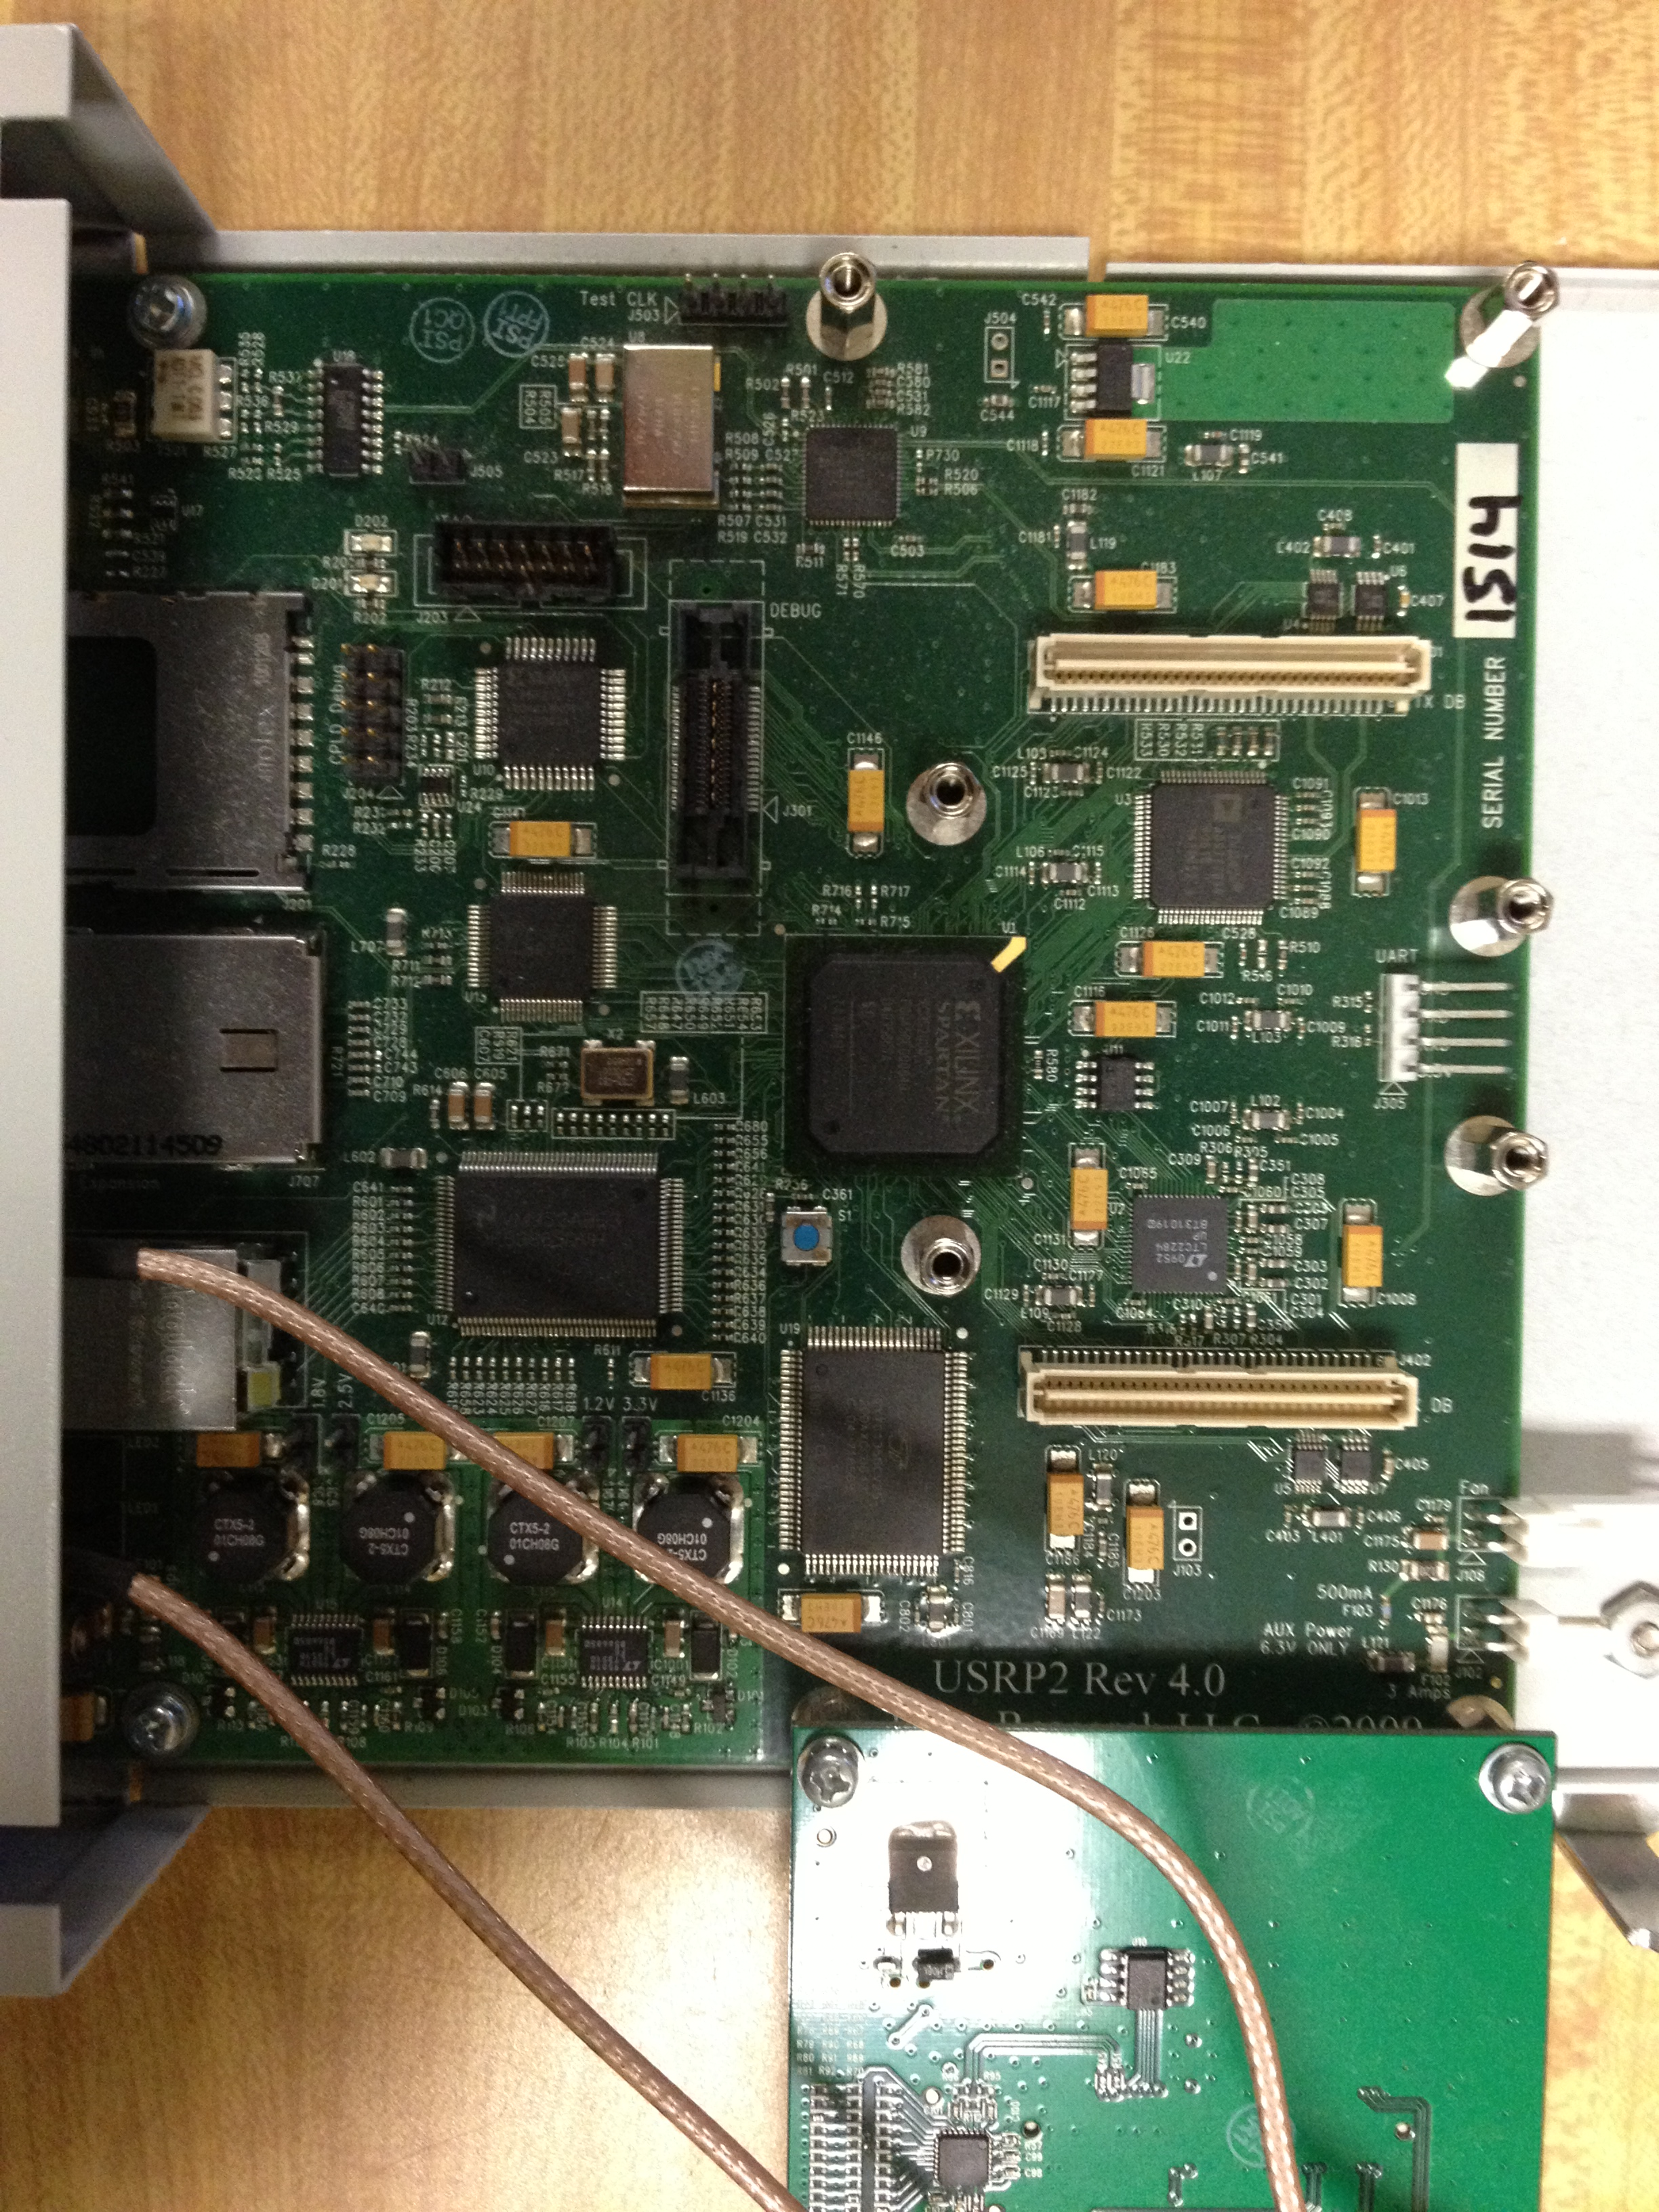
\includegraphics[scale=0.1]{usrp2_mainboard.eps}
%\caption{USRP2 mainboard}
%\end{figure}


The information flow is important to understand within the physical radio.  This SDR block diagram shown below, outlines the common tasks done by the: daughtercard, FPGA, DAC/ADC, and host computer.  Since the FPGA is programmable the operations can change if desired, but the three dominating software packages that utilize the USRP2 follow this structure.  Beginning on the far left of the diagram and continuing to the right, at the daughtercard are RF emissions are received and transmitted.  The daughtercard also contain mixers that translate the signal to an intermediate frequency.  Next come the dual 100 MS/s 14-bit ADCs, dual 400 MS/s 16-bit DACs, two digital down-converters with programmable decimation rates, and two digital up-converters with programmable interpolation rates \cite{USRP2Stats}.  These are located on the main-board of the USRP2 itself.  The FPGA is a Xilinx Spartan 3 XC3S2000, whose current FPGA software is 59\% free in general logic but only 3\% free in memory.  Note that the FPGA also does not have any DSP resources.  The limited memory left in the USRP2 FPGA severely limited any additional development.  As a result, newer models, such as the N210, have an upgraded FPGA \cite{n210spec}.\\

\begin{figure}[!ht]
\centering
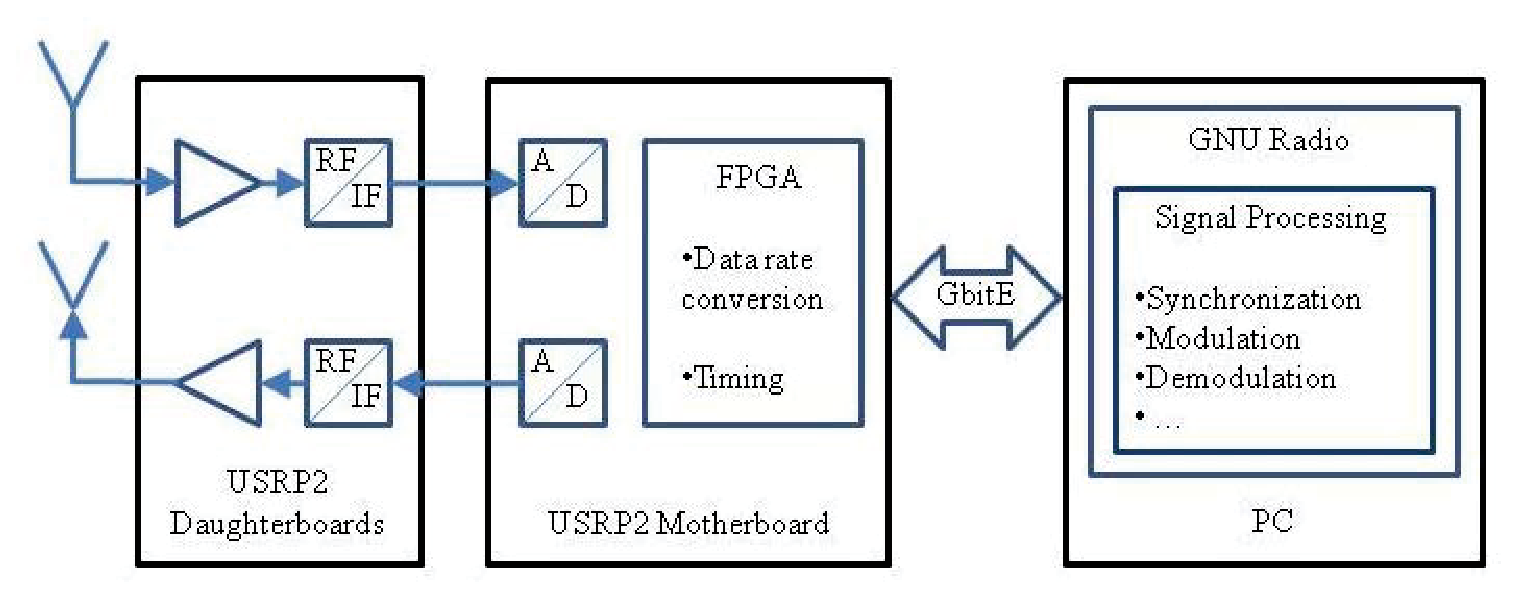
\includegraphics[scale=0.5]{sdr_block_d.eps}
\caption{USRP System block diagram outlining the two operational sections of the USRP itself and their tasks, as well as the PC connected to radio \cite{sdr_blocks}.}
\end{figure}

The data itself contains several pieces of metadata in a frame.  RX metadata structure for describing sent IF data includes time specification, fragmentation flags, burst flags, and error codes. The receive routines convert IF data headers into metadata \cite{metadata}.  Such metadata can be used to indicate the position and FPGA timestamp associated with the sample that corresponds to the start of the underlying frame. By default, existing blocks will transparently propagate any attributes contained on their input streams to their output streams. Blocks that use the attributes can query their input streams to locate all (key, value, offset) tuples in the region of the stream that they are currently working on in their ``work'' method. Likewise, blocks can copy, add or delete attributes on their output streams \cite{sdr_blog}.  This knowledge is extremely useful when doing multiple receive antenna arrays when alignment is necessary, or in any situation where fine timing information is required.\\

With the USRP2 hardware, several software options are available including: GNU Radio, MATLAB, LabVIEW, and several custom solutions.  MATLAB and GNU Radio have already been discussed, therefore the selection between them shall be discussed.  Since this system is a MIMO implementation, signal alignment is a requirement.  At the moment MATLAB does not support sample alignment in a multiple USRP2 system.  Nevertheless, the sample alignment is possible through either external means such as through an external clock or through the option chosen here, the MIMO cable.  The MIMO cable, a picture of it can be seen in Figure \ref{mimo}, is a standard 16-pole flatcable to connect tvrx, basic-rx or dbsrx boards.  Of this 16pin flatcable only two pins are used (io15 and ground) \cite{mimo_cable}.  An image also of the combined dual radio source block can be seen in Figure \ref{mimo_grc} from GNU Radio.  With this requirement GNU Radio must be used for direct access with the USRP2.  As well, full implementation of the systems blocks were first attempted with GNU Radio.  Fortunately, if necessary, data can be passed to MATLAB for signal processing from GNU Radio through the use of the file blocks and a script located in Appendix A.\\

\begin{figure}[!ht]\label{mimo}
\centering
\includegraphics[scale=0.1]{mimo2.eps}%taken on iphone
\caption{USRP2 MIMO Cable}
\end{figure} 

\begin{figure}[!ht]\label{mimo_grc}
\centering
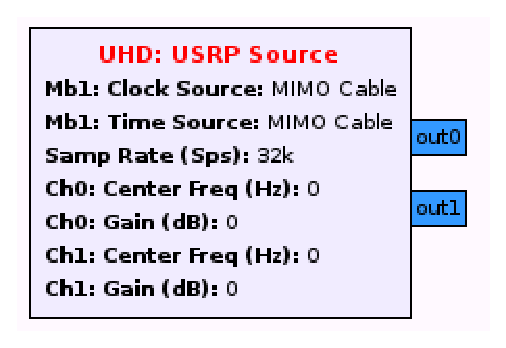
\includegraphics[scale=0.6]{mimo_grc.eps}
\caption{GNU-Radio MIMO Enable Source Block}
\end{figure} 


\section{Spectral Subtraction}

Now that a formal system level approach has been presented and hardware setup chosen, a more detailed understanding of the blocks themselves can be examined.  Spectral Subtraction will be discussed first then the Signal Separation block.  The goal of the Spectral Subtraction block is to removal signals to allow the Signal Separation block to work properly, or to properly recover the desired signal.  As discussed previously signals would first need to be identified and then removed based on information supplied in a precompiled database of known signals.  The technique to remove such signals is called Spectral Subtraction, which primarily takes place in the frequency domain.  This approach only relies on known PSD's of the interfering signal.  All previous research into this topic area was done by Robert Over, using the original definition, providing MATLAB and C++ simulations.  Unfortunately, the C++ simulations, which were designed to be push to the real-time prototype, could not be utilized or adapted because of their incompatible library functions with GNU-Radio.  This research was used as a foundation to provide a viable and implementable solution for Spectral Subtraction.  Initially this technique seemed quite sound, but further investigation proved otherwise.\\

Initial simulations were created to examine this spectral estimation technique at RF frequencies rather than the standard audio frequencies for which Spectral Subtraction is formally used.  Only two signals were used in these simulations, both utilized the same modulation scheme and pulse-shaping filters.  The signals were chosen to be non-orthogonal, since orthogonal signals are inherently non-destructive.  The frequency of the interfering signal was varied, along with the over-subtraction parameter \(\alpha\) and quantization floor \(\beta\).  Through experimentation \(\alpha\) worked best at a value greater than 10, and \(\beta\) worked best between 0.05 and 0.2.  The graph in Figure \ref{SS_basic} shows the bit error rate (BER) as the interferer is shifted across the wanted signal in frequency.\\

\begin{figure}\label{SS_basic}
\centering
\includegraphics[scale=0.5]{SS_basic.eps}
\caption{Original Spectral Subtraction Technique Results}
\end{figure} 

As you can see this spectral subtraction technique operates extremely poor when the signal are overlapping at all.  The reason system performs well at large frequency shifts is due to the bandpass filter which is used before the signal is quantized.  The reason the result is poor is because the estimate is largely incorrect.  Since the subtraction only utilizes the PSD's of the signals, half of the information is completely ignored.  This results in an inaccurate estimate.  The problem with traditional Spectral Subtraction is that its results are subjectively evaluated or done, which isn't accurate enough in a digital communication system.  Other evaluations uses such metrics as SNR, which can be quite deceptive especially in digital communications.  Such examples are covered in \cite{ss_subjective1}, \cite{ss_subjective2}. \\

Since the initial simulations for traditional Spectral Subtraction proved inadequate, other options needed to be explored.  First, the problem needed to be an analyzed further for better understanding, then the appropriate solution could be formulated.  Since the interfering signal and the wanted signal are non-orthogonal to one another they will share dimensional space, in this case the signals are in phase with one another.  Therefore, both planes real and imaginary must be considered.  Non-orthogonal signal removal is a common task in communication system, which is done primarily by equalizers.  Therefore, an equalizer approach was considered next.\\

\subsection{Equalizer Approach}

The equalizer approach used in this Spectral Subtraction approach is a Least Means Square (LMS) equalizer, utilizing training data used in the front portion of each transmitted frame \cite{9}.  This a common equalizer used in practice, allowing for future translation into a realized implementation.  The LMS equalizer was also chosen for it robustness to noise, which is a weakness of such equalizers as the zero-forcing equalizer, and requires no matrix inversion such as the Least Square (LS) equalizer.  For proof of concept the entire data-stream was used as training data, which provides the best results of any given channel for an adaptive equalizer, since the maximum knowledge is gained about the channel for each frame received.  The results below show the BER as the signals pass over one another in frequency, similar to the previous evaluation using traditional Spectral Subtraction.\\
  
\begin{figure}[!ht]\label{SS_equalizer}
\centering
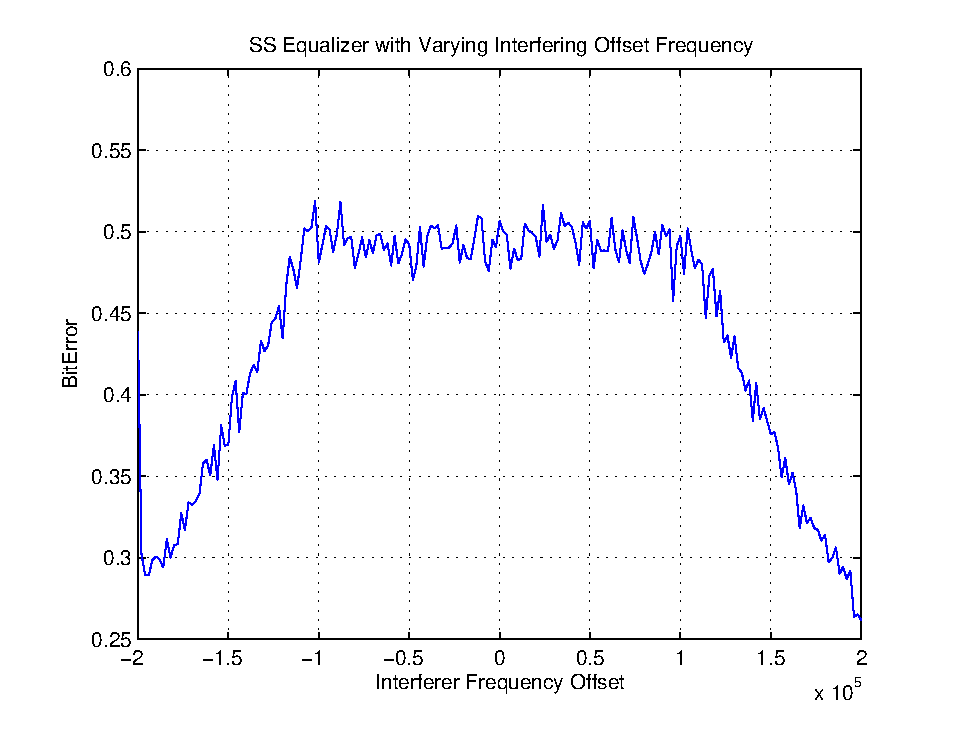
\includegraphics[scale=0.5]{SS_Equalizer_sim.eps}
\caption{Spectral Subtraction equalizer test shifting jammer across a large frequency range, causing overlaps or interference with the desired signal.}
\end{figure} 

As you can see the Figure \ref{SS_equalizer}, the equalizer approach doesn't provide any improvement beyond the traditional Spectral Subtraction approach.  Figure \ref{SS_equalizer} shows massive errors when the frequency of the jammer is within kilohertz of the communicating channel.  The reason the error decreases on the sides of the transmission, is due to the lack of any overlap in the frequency domain of the interferer and the desired signal.  The problem with using traditional adaptive equalizers is that they can only be used with a comparative slowly fading channel.  Since knowledge learned from the training data can be applied at the earliest to the next frame, if the interference changes enough it can render the equalizer useless.  This rapidly changing spectrum or energy within the spectrum is unfortunately a common characteristic of jammers.  Even though this approach failed it provided an important observation and incite into the requirements and scenarios in which jammers can be overcome.\\ %For the sake of completeness an additional test was done with a small repeating sequence, smaller than the equalizer tap size, and as expected the equalizer was able to overcome the interferer.\\

%\begin{figure}\label{SS_equalizer_small}
%\includegraphics{SS_Equalizer_small.eps}
%\end{figure} 


The important conclusion drawn from the previous experiment is that the when signals are orthogonal the receiver needs to be able to predict what data or energy is being transmitted at a given time.  Therefore, the jammer problem must be constrained future.  As a result two jammer conditions will be defined.  The first condition is that the jammer's modulated data or energy is completely known to the receiver and the second is that the data sequence repeats with period being small.  The larger the period the more resources the receiver will need to devote to its determination and evaluation.  The sequence being completely known to the jammer is a reasonable assumption; primarily if the jammer is friendly, as discussed previously in this thesis, then that knowledge can be readily available.\\

Now that the jammer scenarios have been defined further they can be evaluated.  The first will be when the data sequence of the jammer is completely known to the receiver.  The approach here will be to synchronize with the interfering signal, so the interferer will simply be subtracted off.  To synchronize the signals a mathematical tool called correlation will be used.  Correlation is a common tool used in synchronization in communication systems when looking for known symbols in a stream of data.  Equation (\ref{cross}) for cross-correlation simply passes signals over one another, the resulting sequence creates peaks where the data is most correlated.\\

%\[ (f\star g)[n] = summation f^{\star}[m]g[n+m]\] NEED CITATION\\
\begin{equation}\label{cross}
R_{XY}(t_{1},t_{2})=E[X_{t_{1}}Y_{t_{2}}] \cite{gubner}
\end{equation}

An example of two sequences being cross-correlated with one another can be seen in Figure \ref{ss_correlation_ex}, where the larger first signal contains the smaller second signal. The peaks, in red, are the locations the desired signal is most correlated, and the index of these large correlations is the location of the desired signal with the larger mixed signal.  Therefore from this data the location of the start of the interferer's data can easily be located and removed.  A simulation was created with this design in mind, with a unique result.  Since the signals are frequency shifted over one another, when there frequencies match, it produces the best result, but as soon as they are offset, errors start to occur.  This can be compensated for using a complex exponential multiplied by either the received or cataloged waveform.  This will induce a frequency shift canceling out the shifting signal.  Therefore the error will primarily be a function of the noise itself.\\

\begin{figure}[!ht]\label{ss_correlation_ex}
%changing power graph of subtraction
\centering
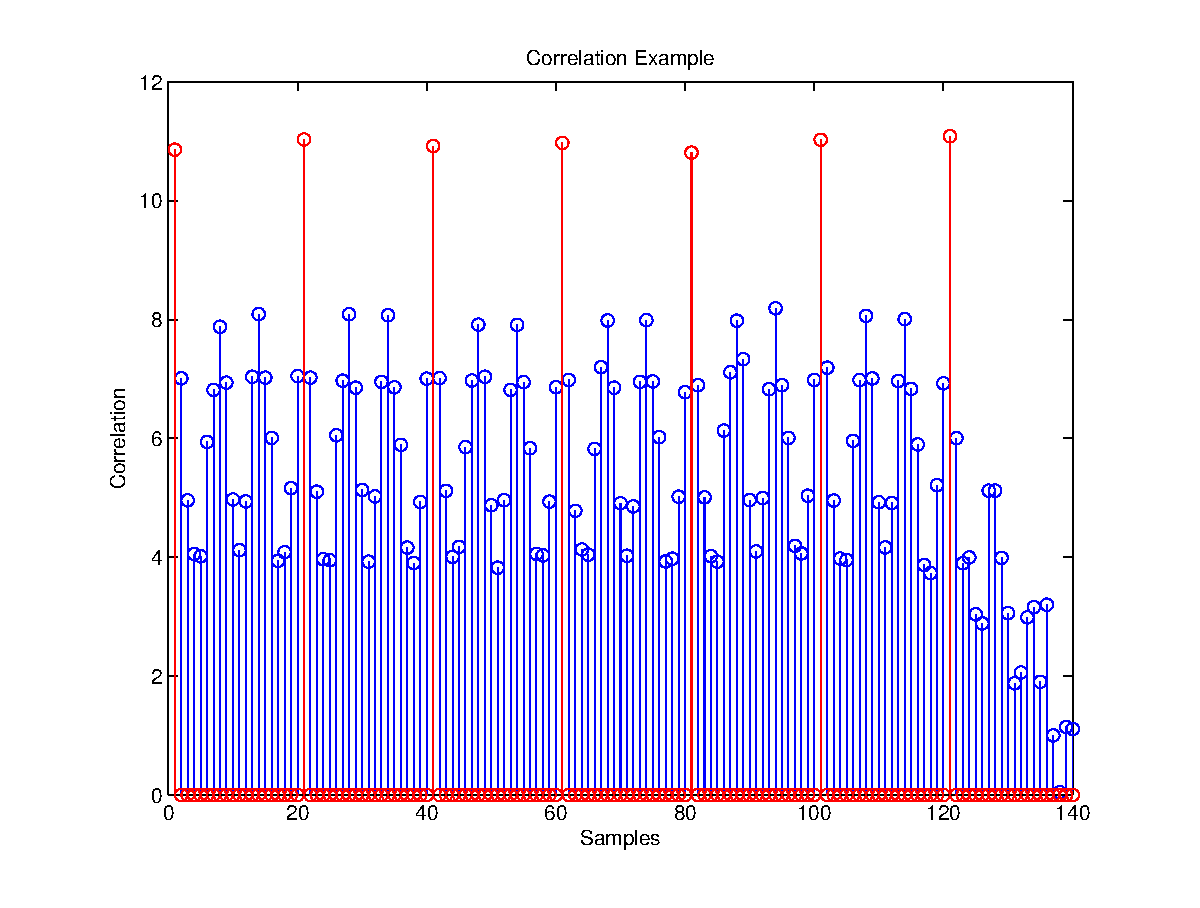
\includegraphics[scale=0.5]{correlation_ex2.eps}
\caption{Autocorrelation of random signal and signal subsection.  The red peaks show the locations of the subsection embedded in the random signal.}
\end{figure} 

\begin{figure}[!ht]\label{ss_correlation}
%changing power graph of subtraction
\centering
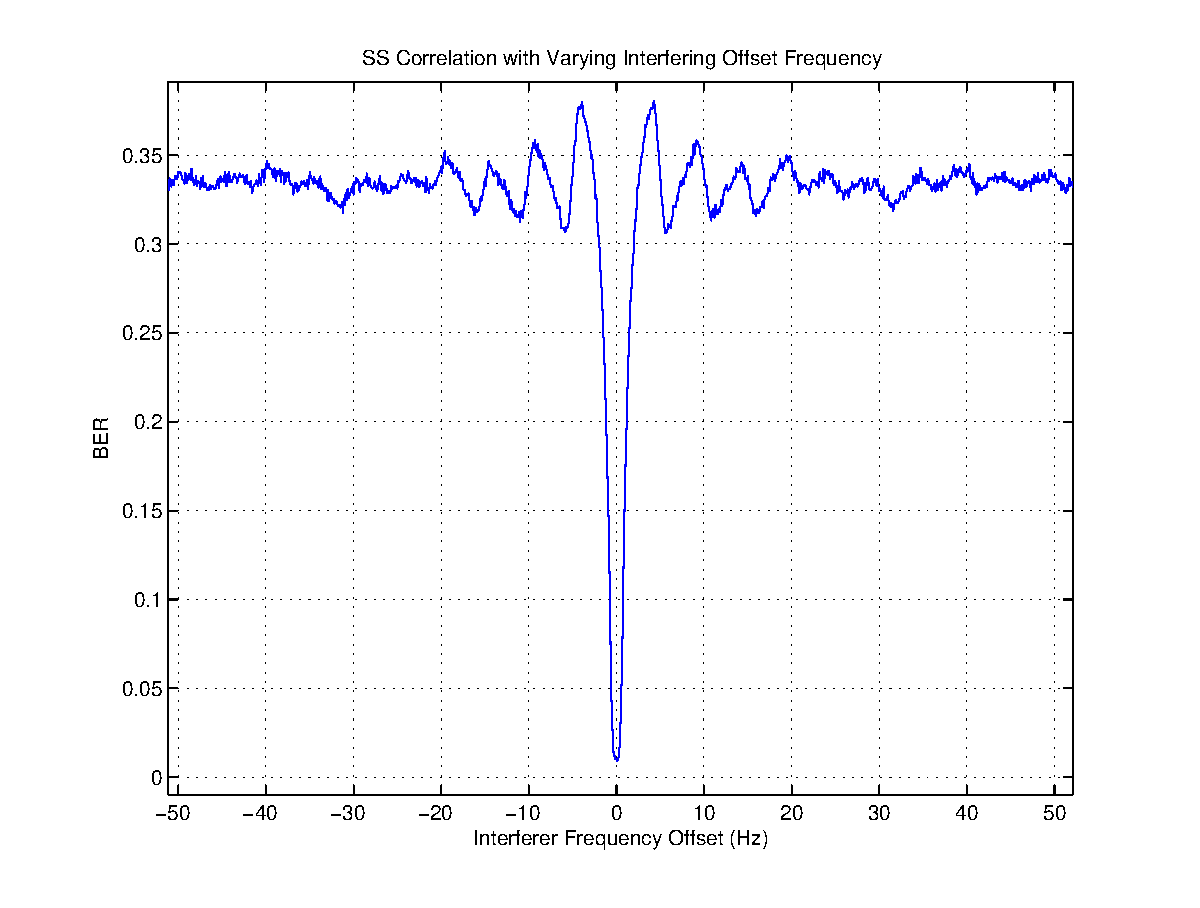
\includegraphics[scale=0.5]{ss_correlation_sim2.eps}
\caption{Spectral Subtraction correlation method, with fixed subtraction estimate frequency and shift actual interferer center frequency.}
\end{figure} 

This simulation was also repeated but with prior knowledge of the interferer's carrier frequency was assumed known.  As expressed previously the subtraction estimate was frequency shift to match the interferer, and then finally subtracted off.  Figure \ref{ss_correlate_GG} shows the overall desired result, with uniform error across all offset frequencies.\\

\begin{figure}[!ht]\label{ss_correlate_GG}
%changing power graph of subtraction
\centering
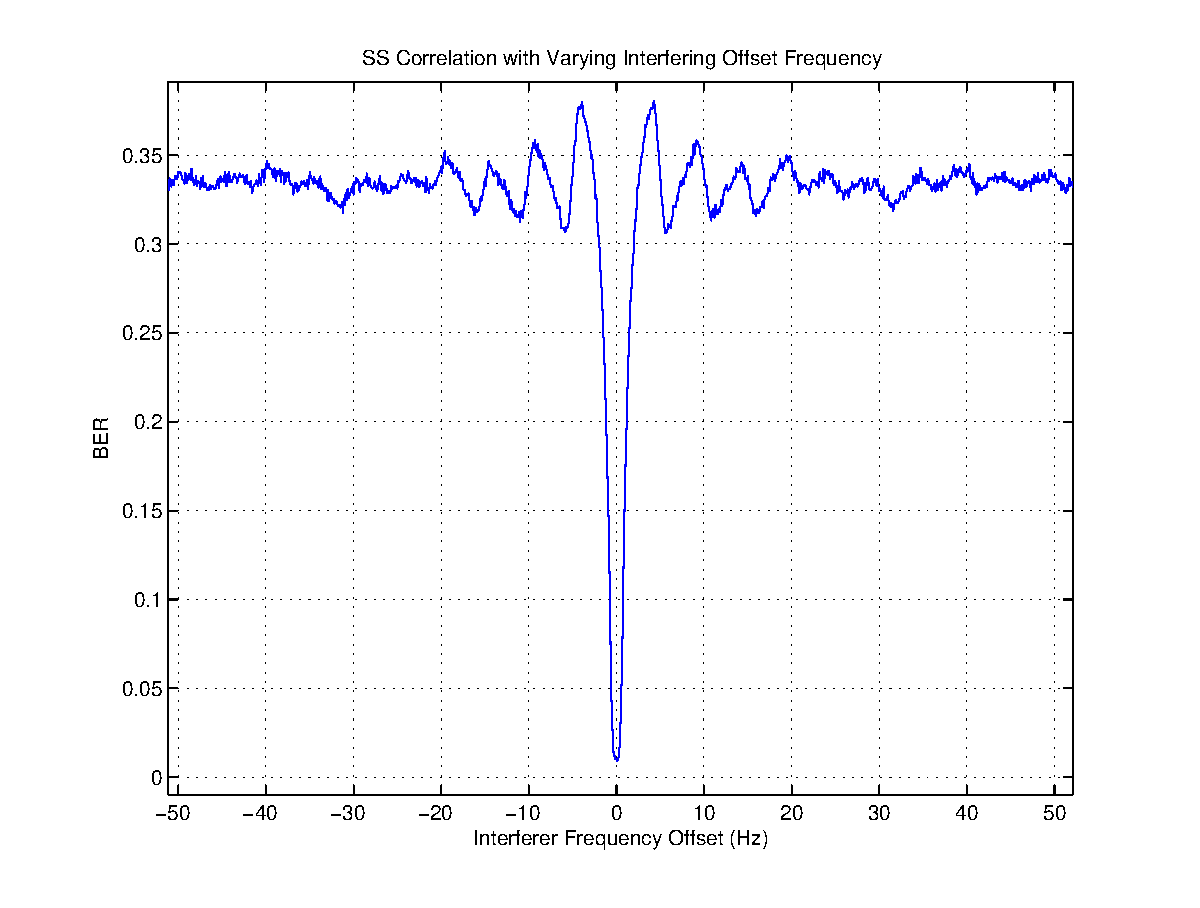
\includegraphics[scale=0.5]{ss_correlation_sim2.eps}
\caption{Spectral Subtraction correlation method, with matched subtraction estimate frequency to shifting actual interferer center frequency.
\end{figure} 

Further analysis was done to provide a solid understand of the new requirements of the system and its limitations.  The first is the precise understanding of the interfering signal itself.  Since it is assumed that the signal modulation and data stream are known, attention can be shifted to the other issues that can occur, which are the non-idealities of the system.  The first is the power constraint or effects.  When subtracting the interferer, accurate power measurements must taken so the estimate is scaled correctly for the environment.  By accurately estimating the power of the interferer, minimal energy will be subtracted from the the desired signal, which is also in the band.  An examination of the incorrect estimation of the interfering signal's power was examined in Figure \ref{fig:power_delta}.

\begin{figure}[!ht]\label{fig:power_delta}  
%changing power graph of subtraction
\centering
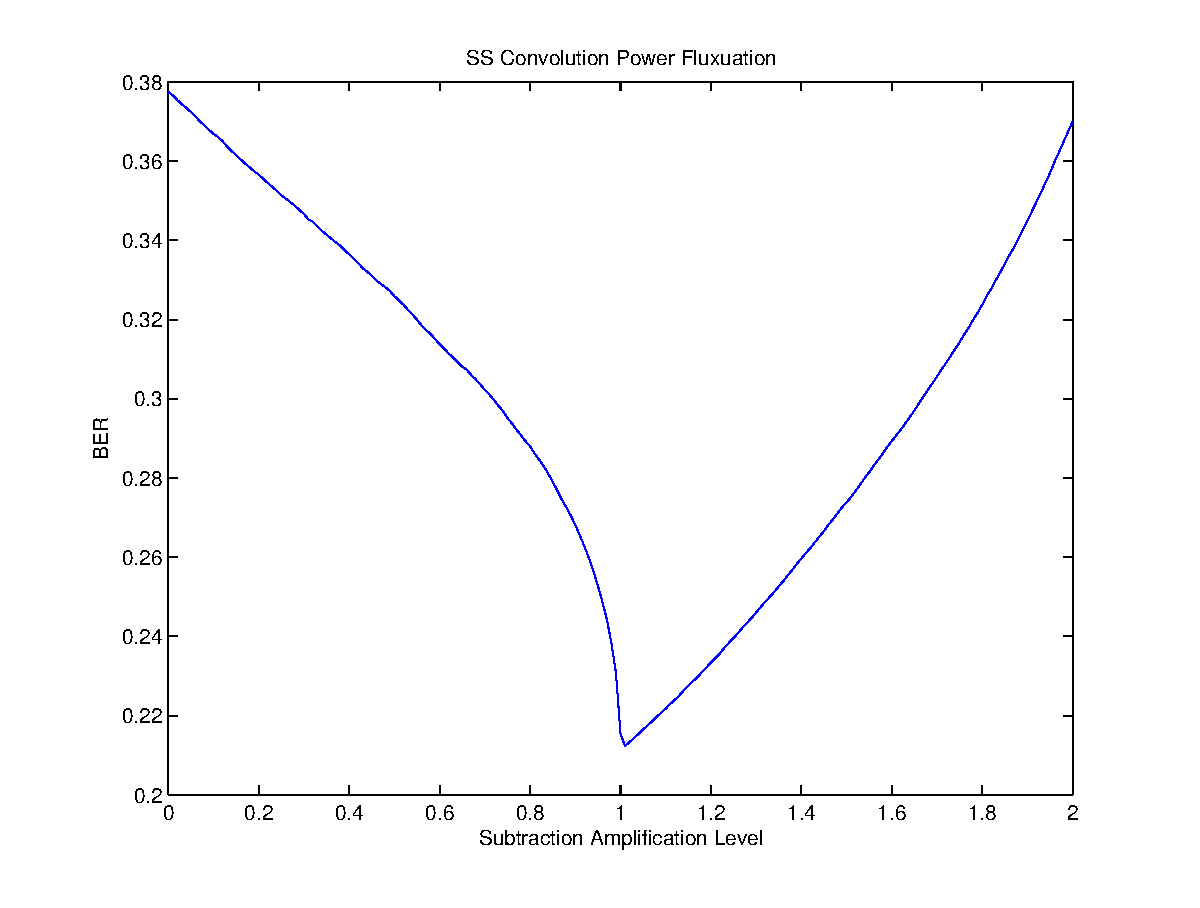
\includegraphics[scale=0.5]{ss_conv_changing_over_subtraction_level.eps}
\caption{Spectral Subtraction correlation test with varying power level scaling interfering signal, while examining the BER of the decoded desired signal.  This shows the sensitive to power difference of the two signals.}
\end{figure}

Besides power, frequency and timing offsets were examined.  These are especially concerning because the signal cannot be demodulated when in operation for feedback information. This is because it must be fed into the signal separation block for equalization.  Therefore a timing recovery mechanism cannot down-sample the signal either.  The timing recovery and carrier recovery mechanism therefore needed to be unobtrusive as possible to the signal.  As a result frequency and timing shifts were examined to understand the sensitivity of the subtraction, and how accurate the recovery mechanism needed to be.

%Freq Shifting
\begin{figure}[!ht]\label{shifting}
%Timing (Phase) shifting
\centering
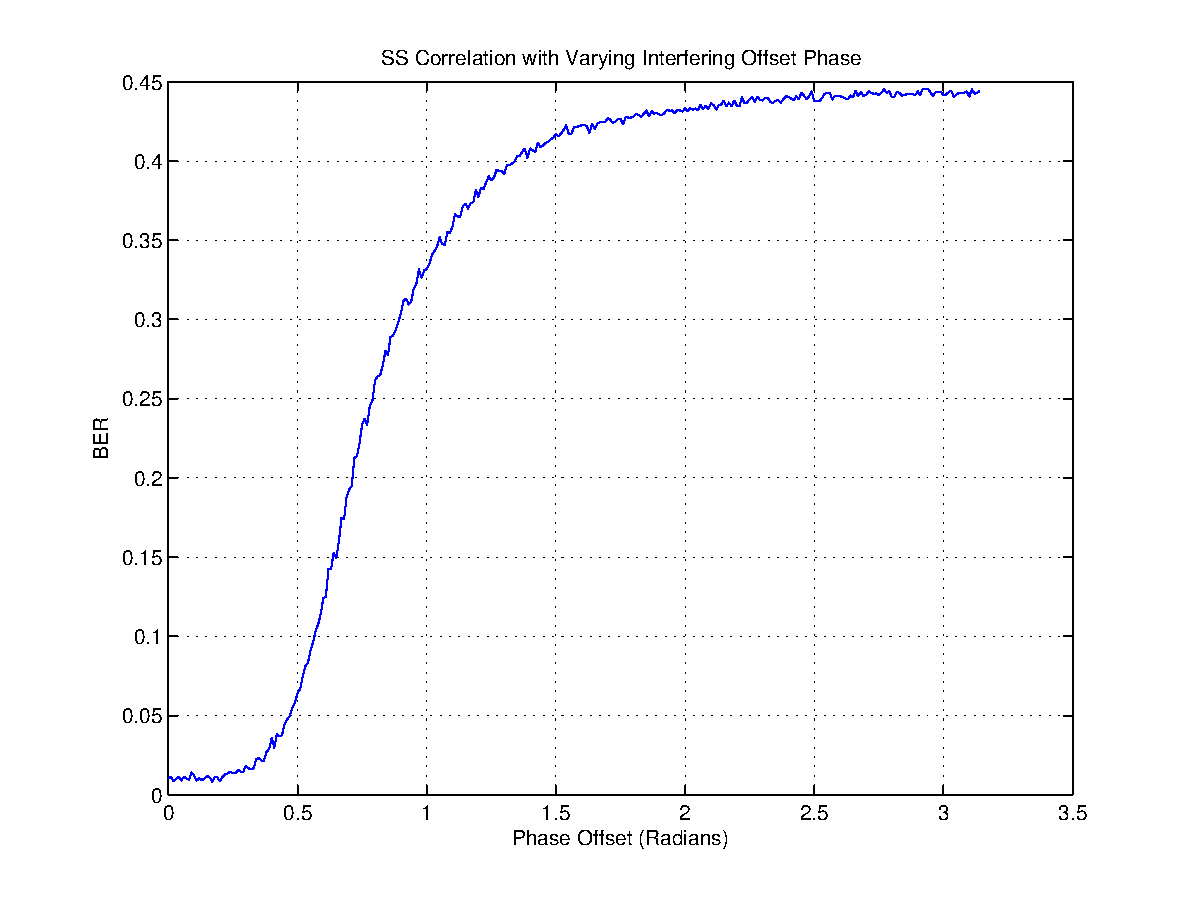
\includegraphics[scale=0.5]{ss_conv_phase_offsets2.eps}
\caption{Spectral Subtraction with phase offsets of interfering signal, showing large error in the decoded desired signal.}
\end{figure}

As you can see from Figure \ref{shifting}, the subtraction mechanism is very sensitive to phase timing offsets.  If a full bit-shift occurs then the entire system falls apart.  This is a rather large problem and must be considered when attempting such operation on non-simulated data.  The frequency sensitivity can be seen from a previous figure, Figure \ref{s_correlation}.  This problem was foreseen because of the time variance or sensitivity of the signals themselves.  Therefore, adaptive compensation methods must be utilize in the final implementation to fix these corruptions.\\

\subsection{Hardware Consideration}

Now that a viable subtraction technique has been determined, the final implementation for the Spectral Subtraction block can be realized.  As discussed in the Hardware and Software Platform section of this thesis, GNU Radio was the first to be examined because of its real-time attributes.  This was quite an involved process requiring many weeks of trial and error.  The first implementation was entirely written in C++, which is the recommended language for signal processing blocks in GNU Radio.\\  

Since C++ within GNU differs from many modern programming styles a code implementation or route was taken to ensure accuracy and speed up development.  Therefore all coding was done with C++ itself, using no GNU Radio built-in libraries \cite{gnuradioCPP}.  To allow for matrix operations the Aramdillo C++ Library \cite{armadillo} was imported and provided needed vector operations such as correlation and faster mathematical functions instead of having to rewrite common search operations.  This library would also be needed for the Signal Separation block, therefore coding with Armadillo would provide the knowledge for future implementations needed in that block.  From the standard C++ implementation results were compared with MATLAB, and the code was ported into GNU Radio.\\

\begin{figure}[!ht] 
\centering
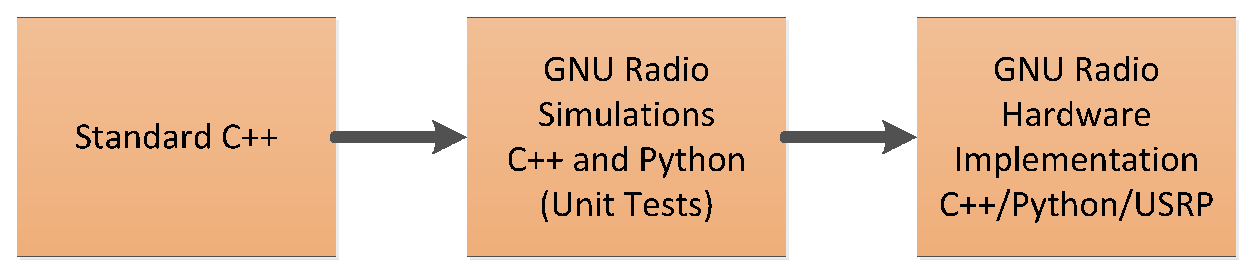
\includegraphics[scale=0.5]{code_work_flow.eps}
\caption{GNU-Radio code implementation workflow}
\end{figure}

GNU Radio C++ are basically written by first creating test cases and writing your code until they are solved.  This is a common practice among the programming community and provides a definitive endpoint to the code itself.  The code was written and compiled successfully but unfortunately the python wrapper called SWIG \cite{swig}, which GNU Radio uses to interact with the C++ block through python, was unable to export the library.  This is an undocumented problem within GNU Radio and was only identified through discussions directly with the GNU Radio core development team.  Therefore another approach had to be considered.\\

The next option was to use python itself for signal processing.  This is approach was primarily developed by Josh Blum, one of the core developer of GNU Radio.  It isn't recommended due to speed issue, but it is quite easier to implement and debug for those familiar with python.  As a result the previously C++ code was ported to python standards libraries and then to GNU Radio.  The NumPy libraries were used within python.  NumPy is the fundamental package for scientific computing in Python \cite{numpy}.  It like the armadillo library provides matrix operations such as correlation.  Again under the Python standard libraries with NumPy the results were verified with MATLAB.  Then the code was port to GNU Radio.\\

Again more problems occurred, which inhibited progress.  The signal processing block was written as a subprocess using the queuing system built into GNU Radio.  Queuing provides barriers between the connected blocks.  Therefore they can run freely, limiting bottlenecks. The system built would operate correctly for several hundred samples but would eventually segmentation fault.  Several attempts to fix this error with even architectural changes to the code.  Finally the lead developer of GNU Radio was consulted, Tom Rondeau \cite{tomrondeau}, but he was also unable to determine a solution.  The assumed problem was a type casting occurring within the queue itself, that would eventually accumulate and cause a segmentation fault.\\

With these setbacks, it became necessary to look beyond GNU Radio and utilize MATLAB for signal processing.  Therefore the decision to load captured signals from GNU Radio and process them in MATLAB.  Although not real-time, but this configuration would process the data appropriately.  The simple GNU Radio needs front-end is important because it allows tight synchronization between multiple receive antenna, which is a require of the original design of the system.  The GNU Radio model can be seen in Figure \ref{ref:grc_receiver}, the modulator block has been customized to remove the quantization, producing floating point results.\\

\begin{figure}[!ht]\label{ref:grc_receiver}
\centering
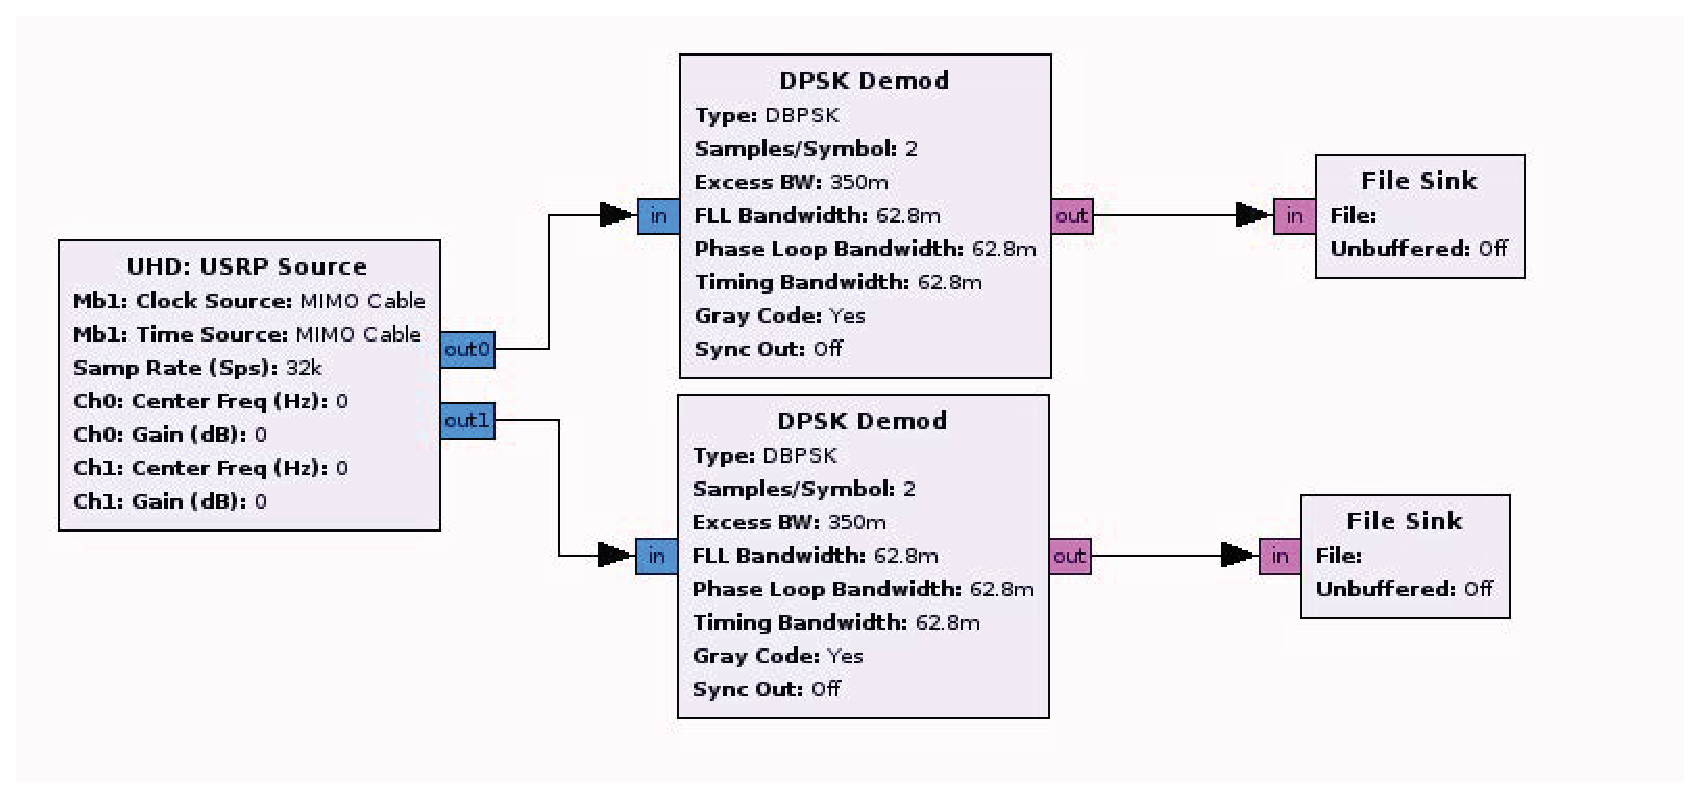
\includegraphics[scale=0.5]{grc_receiver.eps}
\caption{GNU-Radio Receiver Half Design}
\end{figure}

\subsection{Non-deterministic Scenarios}

For completeness it is important to discuss the scenarios when the interferer's modulated data is unknown but repetitive with a small period.  The approach to estimating short sequences is a rather obvious one, an autoregressive algorithm is used to predict samples.  The simulation here, which was just used for proof of concept, uses a linear predictive filter.  The filter determines coefficients of a forward linear predictor by minimizing the prediction error in the least squares sense\cite{lpcfilter}.  It finds the coefficients of a \(p\)th-order linear predictor (FIR filter) that predicts the current value of the real-valued time series \(\textbf{x}\) based on past samples.

\[ \hat{x}[n]=-a(2)x(n-1)-a(3)x(n-2)-...-a(p+1)x(n-p)\]

For the linear predictive filter to operate effectively the number of filter taps must be equal to or greater than the period of the repeated sequence.  If the number of taps is smaller it cannot capture the randomness the in the interferer's data.\\

\subsection{Over the Air Implementation Considerations}

When moving towards a real implementation of the Spectral Subtraction block, the non-idealities introduced by the environment needed to be considered.  These include frequency and phase shifts, as well as timing offsets.  Certain considerations needed to be made as well, since instantaneous changes occur when signals overlap.  Therefore a more advanced control scheme needed to be constructed around the common signal compensation or correction.  The basic idea used here is a receiver within a receiver, one for each signal received.  This will be discussed in detail.\\

The system assumes that the jammer is always present within the environment therefore it was concluded that the jamming signal should be synchronized with first, be removed and then all that remains should be the wanted signal.  There is were the receiver within a receiver design comes in, since first the interferer will be synchronized to, utilizing phase and frequency recovery and then timing recovery.  Unfortunately such an implementation isn't as straight forward as expected.  Since when both signal are present in the spectrum it is impossible for these algorithm to operate correctly.  This is due the fact that they cannot separate one signal from the other.  For example, phase information cannot be accurately calculated in the presence of two signals.  Therefore modifications need to made, which is where a controlling mechanism comes into play.\\

When multiple signals are in the environment the compensation algorithm learn incorrectly; as a result, a decision was made to pause these algorithms when both signals were present and continue when the signal interferer was only present.  This operation relies on two assumptions, the first is that both signals are present for short periods of time which can be controlled.  The second is that the calculated offsets of cause by the environment don't rapidly vary during the periods of time for which the two signals are visible.  This assumption is quite reasonable especially with relatively non-mobile transceivers, which was assumed in the original documentation.\\

To accomplish this algorithm holding mechanism, energy detection was chosen to be uses for its simplicity.  Below you can see an image of the jammer signal by itself and the combined signals.  A large increase in energy or step can be seen, which can easily numerically detected.  Energy is calculated using the following equation: \(E_{s}=\newcommand{\inftyint}{\int_{-\infty}^{+\infty}}|x(t)|^{2}dt\).  This was implemented with a moving average filter with a small window to reduce spurious changes due to signals gaps or outliers.  In practice the average peak energy level of the interferer is first calculated, then when the power in the spectrum increases to a level roughly 1.5x of the original level, the compensation algorithms are halted.  A simple technique, which is commonly uses but in the inverse fashion.  An example of the combined and signals can be seen in Figure \ref{fig:combo_signal_time}.\\


\begin{figure}[!ht]\label{fig:combo_signal_time}
\centering
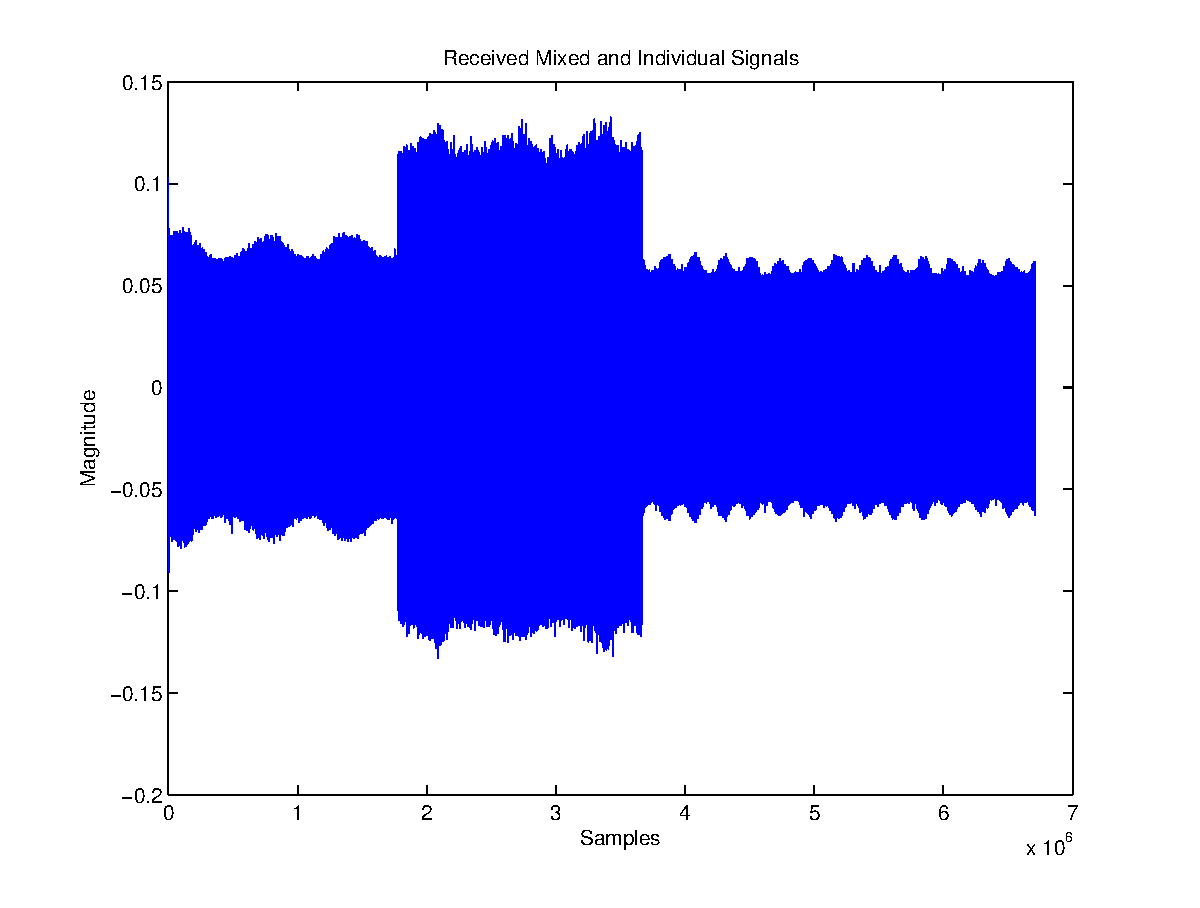
\includegraphics[scale=0.4]{combo_signal_time.eps}
\caption{Sample periods of time when the interferer is only transmitting, both interferer and desired signal is transmitting, and the desired signal alone.  Energy detection can easily determine periods of signal mixing and non-mixing.}
\end{figure}


Now that the triggering mechanism for halting the algorithms has been determined, further detail must be given to the front or subtraction receiver part of this block.  To help replicate the effects of the channel on the subtraction estimate, first a channel estimation is done using the interferer's actual data symbols.  Therefore the received signal is goes through carrier recovery using a signal PLL.  Then using the Mueller Muller method, the symbols are timing recovered and demodulated.  This data is then fed through a LMS adaptive filter and a channel estimate is produced.  Using this channel estimate, a pre-generated known interferer waveform is filtered after passing through an Automatic Gain Control block. This normalizes the previously known signal with respect to the received one.  Next the signals are aligned using the correlation method examined previously, and the first found frame in the received signal is copied from that signal.  This section is then duplicated to the size of the full received stream at a given time, then finally the two are subtracted from one another.  Since the received signal cannot be demodulated or quantized before it reaches the Signal Separation block, all subtractions are done on the baseband received signal.  The final results of the Spectral Subtraction block are examined in the next chapter.\\

\begin{figure}[!ht]\label{ss_overview}
\centering
\includegraphics[width=1.1\textwidth]{SS_overview.eps}
\caption{Spectral Subtraction Block Diagram}
\end{figure}


\section{Signal Separation}

The next block to discuss is the signal separation block.  The development of this block is very staggered and due to time requirements shortcuts needed to be made.  The original desired result was to use a blind source separation technique outlined here \cite{AMUSE}, which is able to separate multiple signals from one another under specific constraints.  %For this process to operate effectively an appropriate channel model needs to be created.  Since the goal of this system is to be very robust an estimator for very frequency selective channel is desired.  The progression of the signal separation block will be examined in this sections and the limitations will be discussed.  It is important to note that a large variation was taken in the system design due to implementation feasibility.\\

Instead of utilizing a AMUSE, it was decided a new avenue was to be taken, with a more theoretical channel estimation problem in mind.  The primary investigator here was Dr. Srikanth Pagadarai.  He focused on deriving a MIMO co-channel correlation model, by utilizing Superimposed equalization to acquire channel information.  His goal was to provide a method of channel estimation for a MIMO channel mixing problem by utilizing shared channel information.  Primarily focusing on training symbols themselves.  It it important that this research be discussed here, since it received the most attention of all three of the AS\textsuperscript{6} blocks.\\

The first objective for channel estimation is to examine the channel mixing model which assumes a single-input multiple-antenna broadcast channel.  A J-channel FIR system excited by \(K\) transmit antennas is considered. A quasi time-invariant multi-path channel is assumed which remains constant during the transmission of a set of consecutive symbols, which are called slots. These slots are assumed independent from one another.  The channel estimation is performed over each slot. Each symbol inside a slot is assumed to be the result of a known redundant precoder acting on an input transmit symbol vector drawn from an M-PSK constellation. Therefore the receiver receives signals not only from the intended transmitter but also from \(Q\) other interferers. The interferers are assumed to employ the same redundant precoder as the desired signal \cite{skrkantPHD}.\\

With this model, reference \cite{midterm_report} shows that no assumptions are necessary regarding the number of the transmit antennas of each of the interferers and the channel orders as long as they are smaller than the block size.  The block size in this case is equal to the combination of the individual channel lengths and the number of transmit antenna used by the desired transmitter.  But this evaluation rely on three assumptions:

\begin{enumerate}
\item The data sequence \(x_{d}\) is an i.i.d. sequence such that \(x_{d}\sim\mathcal{CN}(0,\sigma_{d}^{2})\).

\item The distribution over the MIMO channel vector is \(p(y;\theta)\sim\mathcal{CN}(\mu_{y},R_{w})\), and the interference vector is distributed normal with covariance \(R_{w}\).

\item The transmitted symbols, the channel vector, and the interference vector are jointly independent.
\end{enumerate}

With these assumptions the mixing process can be undone but the channel estimation needs to be calculated first.  Since this is a MIMO channel, frequency selective fading will need to be captured to providing appropriate channel knowledge.  To accomplish this, the original research decided to utilize superimposed equalization, whose operation was heavily discussed in the background section of this thesis.  In summary, \cite{Ghogho} uses a superimposed symbol transmission scheme to estimate frequency-selective channels. Several points of the DFT of the data are set to known values. This operation can be easily implemented in the time domain when these DFT points are equi-spaced. The channel is estimated using the DFT of the received signal at these selected DFT points. The detection itself is done using an iterative method across these points.  Unlike traditional equalizers, the proposed method does not require bandwidth for training.  It instead trades spectral power for those symbols themselves, spreading its energy over the entire bandwidth capturing the entire spectrum space.  Reference \cite{Ghogho} also proves that by placing the training symbols in quasi-periodic position they will not interferer with the data itself.  It is important to note that this research discusses no synchronization mechanism, and now with the training data spread throughout the signal is very complex.  This addition complexity was factored into the design decisions of the implementation, which is discussed later in this section.\\

With our channel estimation method chosen, a simulation was created to prove the effectiveness of such a scheme.  The result of this implementation were directly compared with the results of the paper to prove correctness.  % and compared with traditional equalizer performance&
The results of this simulation are seen in Figure \ref{sie}.  It examines a random frequency selective channel, with very high suppression with a across a number of SNR values.  As expected there is a linear relationship between SNR and MSE.\\  %For completeness a comparision was done with a traditional LMS equalizer to show the effectiveness of the superimpose equalizer.\\

\begin{figure}[!ht]\label{sie}
\centering
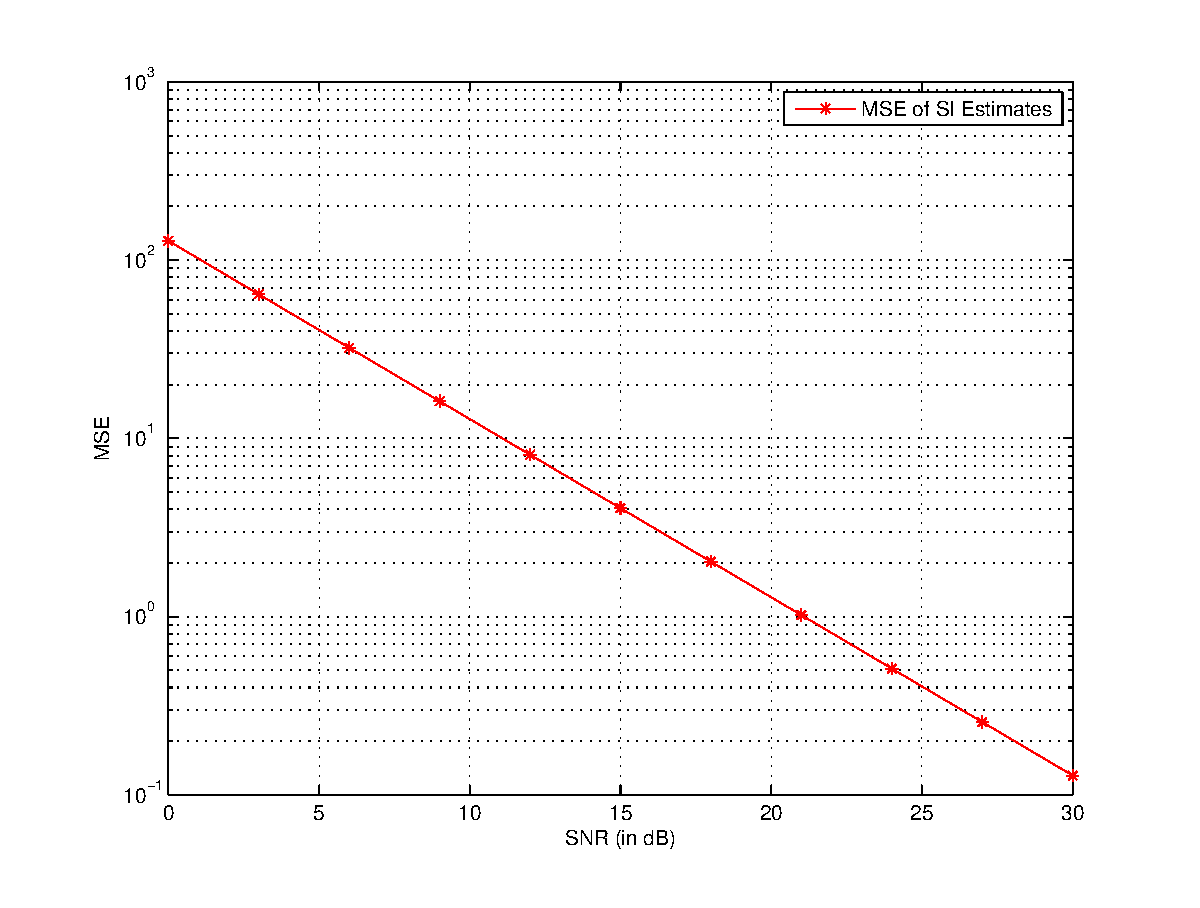
\includegraphics[scale=0.5]{sie_SNR2.eps}
\caption{Superimposed Equalizer MSE across several SNR values.  The clearer the signal the better our estimation becomes.  This result was identical to reference \ref{Ghogho}.}
\end{figure}

\begin{figure}[!ht]\label{fig:sie_freq}
\centering
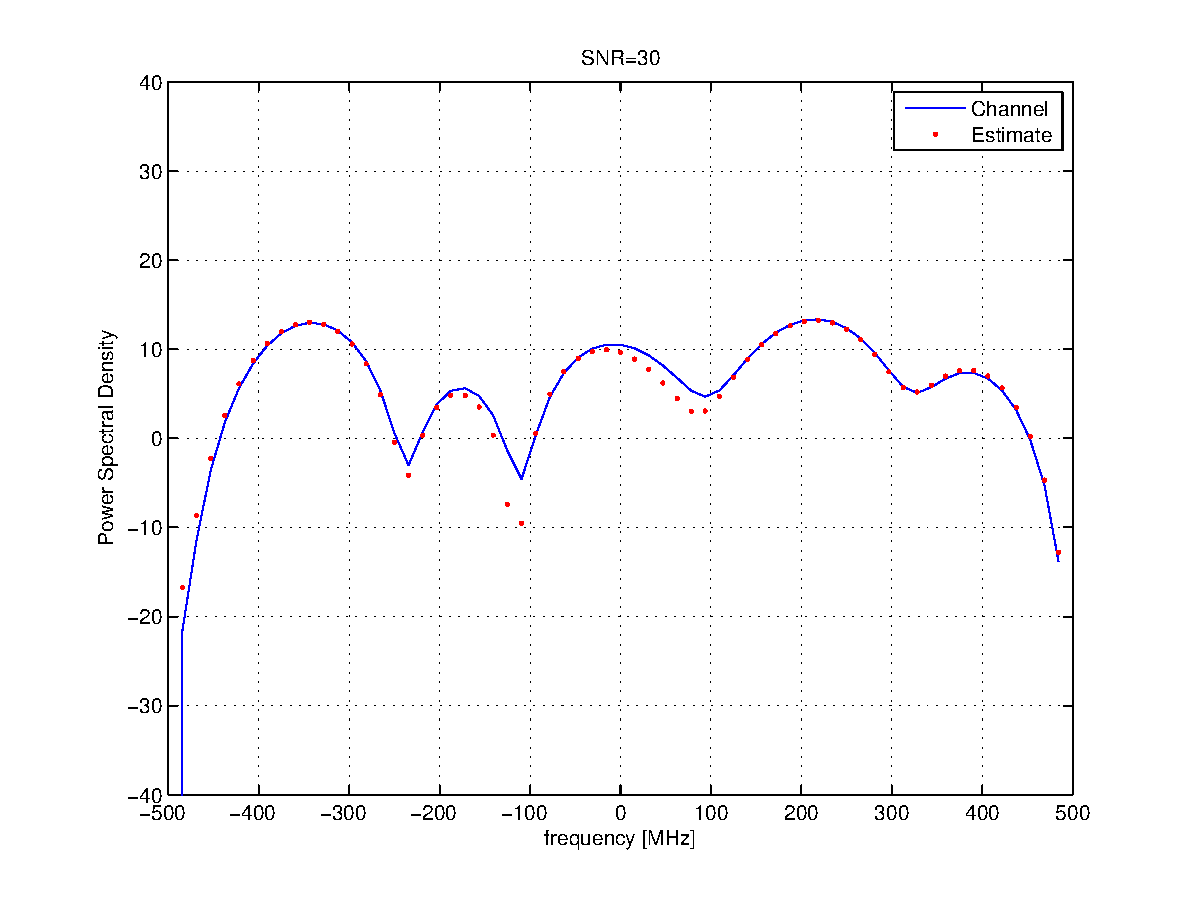
\includegraphics[scale=0.5]{freq_response_sie2.eps}
\caption{Superimposed Equalizer channel estimate superimposed on actual channel.  With SNR > 25, estimates are considered accurate.}
\end{figure}

%INSERT Figure of SNR and channel estimate for Superimpose equalizer\\
%
%INSERT Figure with comparision of superimposed equalizer vs. traditional linear equalizer\\

From Figure \ref{fig:sie_freq} you can see in a frequency selective fading channel is very well estimated by the superimposed equalizer.  This was exactly the result that was desired, but symbol recovery after equalization still needed to be examined. This unfortunately is the drawback of this formulation.  The first is the condition if the mixing matrix \(H\) is rank deficient, the channel become inestimable,  since there become an infinite amount of solutions to the actual unmixing process.  The second is the equalizer, which is numerically intensive, and the alternative has limiting conditions \cite{Ghogho}.  This conclusion, which is not discussed in \cite{Ghogho}, is when the equalized signal is very suppressed due to the incomplete channel estimate.  The quantization feedback method overcome the previously received frame and dominated all future frames, essentially neglecting any information they have.  Again, this only in very suppressive channels.  With these results the superimposed equalizer started to become less desirable due to its complexity, but evaluations continued due to the amount of time invested into the topic already.\\

%NEED MORE MATHEMATICAL EXPLAINATION 


%%%%%%%%%%CONTINUE EDITING
%%%%%%%%%%CONTINUE EDITING
%%%%%%%%%%CONTINUE EDITING

These simulations provide the necessary foundation to push towards the final implementation of the signal separation block.  However, due to time constraints certain decisions needed to be made about this block and the feasibility of its operation.  With that in mind the primary goal for the signal separation block was to provide signal separation or maximization from several received signals.  Since the previous research provided substantial implementation considerations and issue, a new direction needed to be considered.  Therefore instead of the proposed AMUSE \cite{AMUSE} technique, another MIMO cross-channel technique called Maximal Ratio Combining (MRC) was chosen as an alternative.\\

Maximal Ratio Combining is a method of diversity combining in which the signals first weighted, based on their SNR value, and then added together.  These weights or gains are made proportional to the RMS signal level and are inversely proportional to the mean square noise level in that channel, and the same proportionality constant is used for all channels \cite{fs1037c}.  Therefore the channel with the best SNR provides the greatest impact on the resulting sequence. Figure \ref{fig:MRC} outlines MRC with \(N\) input signals.  First the symbols are weighted then simply summed based on this weighting.\\

Assuming the received signal is an array of samples received the individual antennas \(\boldsymbol{x}(t)=\boldsymbol{h}(t)u(t)+\boldsymbol{n}(t)\) and the individual channels \(\boldsymbol{h}=[h_{0},h_{1},...,h_{N-1}]^{T}\), and the additive noise \(\boldsymbol{n}=[n_{0},n_{1},...,n_{N-1}^{T}\).  The equalized symbol \(\hat{x}=x+(h^{H}n)/(h^{H}h) \) \cite{diversity}.

\begin{figure}[!ht]\label{fig:MRC}
\centering
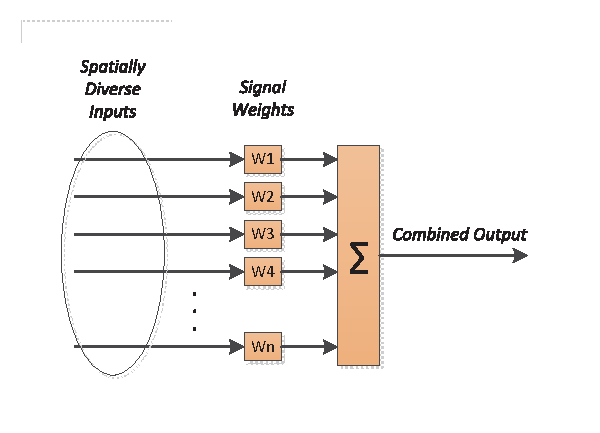
\includegraphics[scale=0.5]{MRC_Sys2.eps}
\caption{Block diagram of Maximal Ratio Combining, which combines spatially separated signals weighted by according to their SNR values.}
\end{figure}


A simple evaluation of MRC was done to prove its capabilities, which is based on the simulations here \cite{mrc_m}.

\begin{figure}[!ht]\label{mrc_sys}
\centering
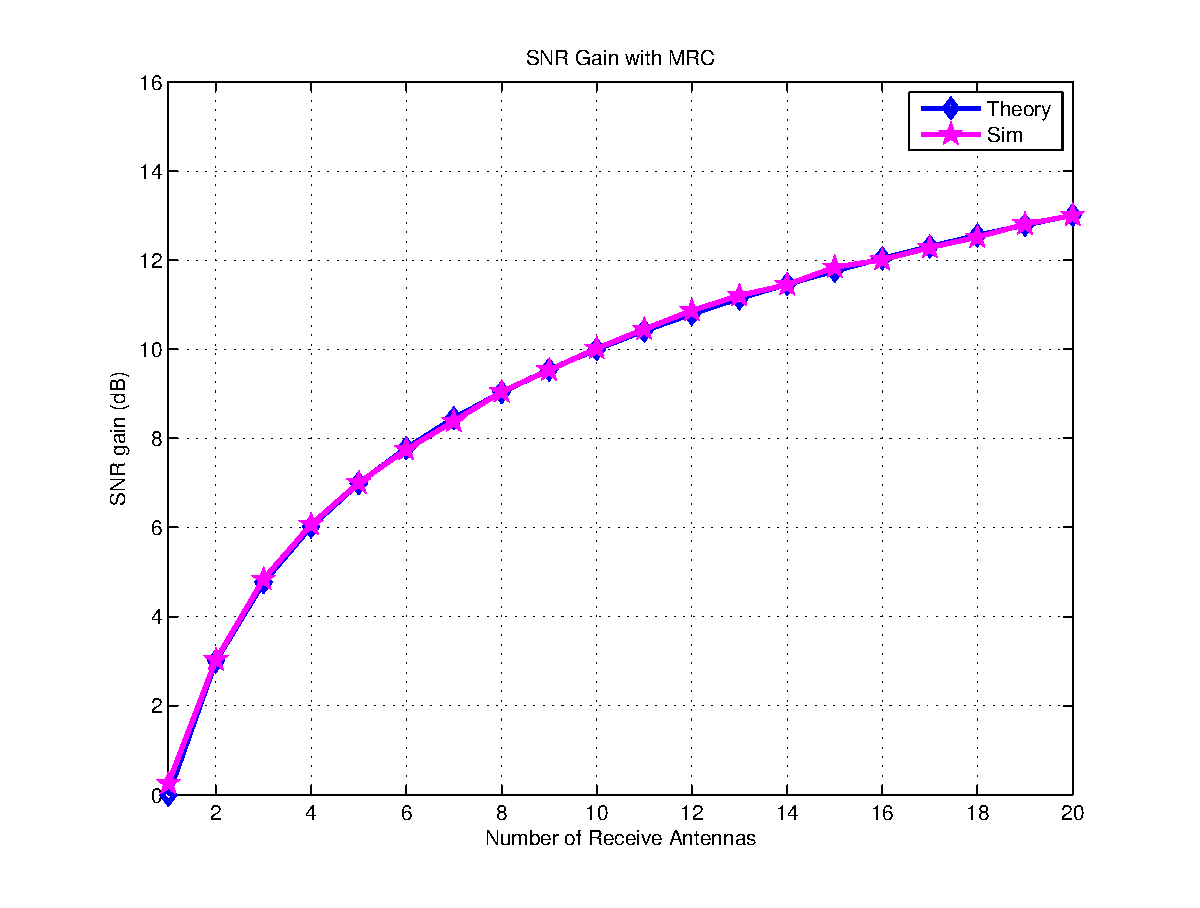
\includegraphics[scale=0.5]{mrc_gain.eps}
\caption{Maximal Ratio Combining gain across varying number of antennas.  The more antennas provided at the input the more spatial diversity, resulting in a higher combined SNR.}
\end{figure}

As you can see as you increase the number of antennas in a frequency selective channel the better the result.  Therefore MRC was introduce into the framework of the signal separation block, and the new model for this block can be seen in Figure \ref{mrc_sys_ss}.  This block first utilizes adaptive equalizers on the channels individually then uses MRC to combine there results maximizing the SNR of the desired signal.  MRC was combined with the channel estimate approach using adaptive equalizers due to there known feasibility.  From the knowledge learned in the previous with the implementation involving GNU Radio, the signal separation block was created entirely in MATLAB.  The results of this operation will be discussed in the final chapter of the thesis.\\

\begin{figure}[!ht]\label{mrc_sys_ss}
\centering
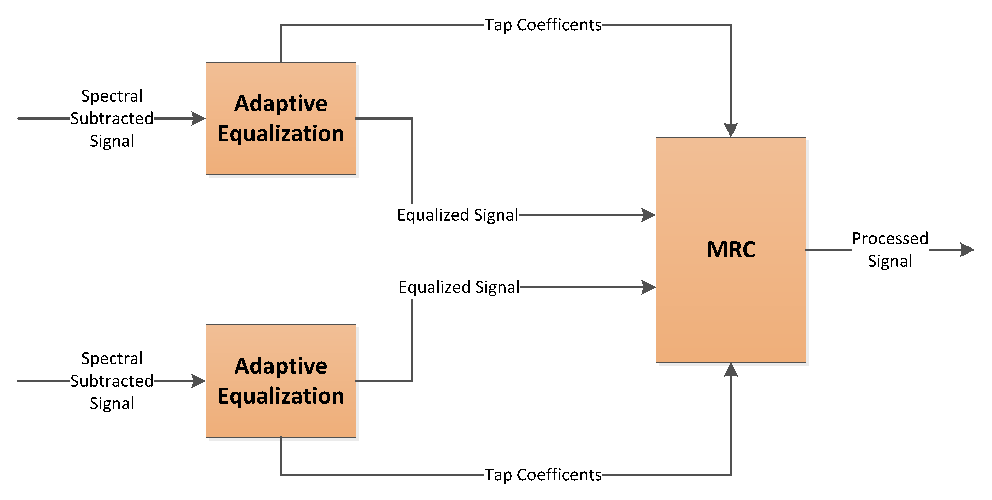
\includegraphics[scale=0.8]{mrc_sys.eps}
\caption{Maximal Ratio Combining block design to replace original Super Imposed Equalizer design.  AntSS currently is only designed to supply two signal, but could be modified for future implementations.}
\end{figure}

\section{Antenna Subset Selection}

The Antenna Subset Selection (AntSS) block was partially implemented by a research collaborating team but was never fully completed.  It is important to understand the purpose of this block for future research, and how it should interact with the other blocks of the system.  The AntSS system itself consists of a series of AntSS boards that provides \(2^{M}$$ -to-$$2^{N}\) down-selection from an array of receive antennas to a set of BLISS receiver inputs. Each individual AntSS board provides 4-to-2 antenna down-selection via a set of RF switches. A basic block diagram of an individual AntSS board is given in Figure \ref{ants_sys}.  Each AntSS board has four receive paths. Each path consists of a bandpass filter and low-noise amplifier. The output of each receive path is connected to a switch matrix composed of a series of Single-Pole-Double-Throw (SPDT) RF Switches. The switch matrix is configured so that all possible permutations of the 4-to-2 down-selection are possible. The switch matrix is controlled by software running on a simple PIC processor. The PIC interfaces with the BLISS hardware platform via an RS-232 link that is connected from the BLISS receiver to all AntSS boards.\\

\begin{figure}[!ht]\label{ants_sys}
\centering
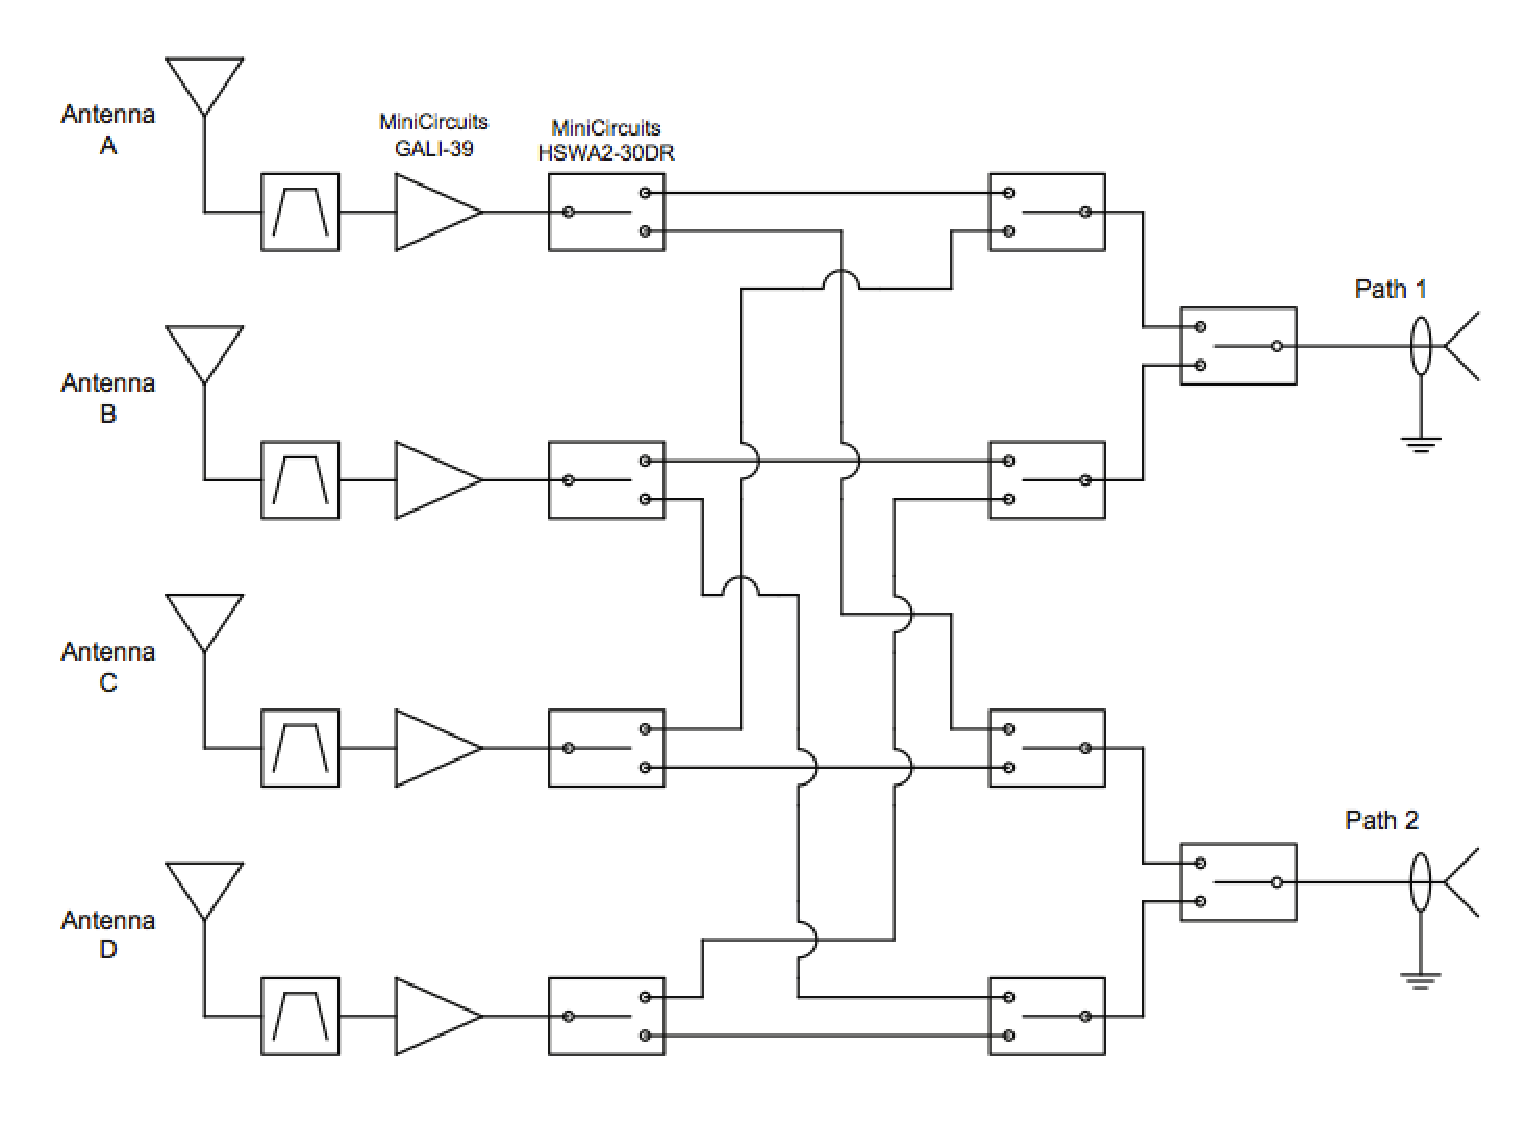
\includegraphics[scale=0.6]{ants_sys.eps}
\caption{Antenna Subset Selection block outline}
\end{figure}

During operation, training information which was used also by the signal separation block is also used by AntSS.  It uses this data to provide SNR values at each Antenna of the desired signal.  Once all antennas have been evaluated the system then selects a subset of the best antennas, which is defined by the highest SNR levels.  The signals from these antennas are then fed into the remain BLISS blocks.  AntSS can have \(2^{M}\) antennas, but will always deliver two signals.  The antennas need to be space at least a single wavelength apart or they will not be considered independent of one another, reducing the effectiveness of AntSS.  The physical boards have been built, which can be seen in figure \ref{antss_boards} and their frequency response on the individual channels can be seen in Appendix \ref{ANTSS_F_RESPONSE}.\\

\begin{figure}[!ht]\label{antss_boards}
\centering
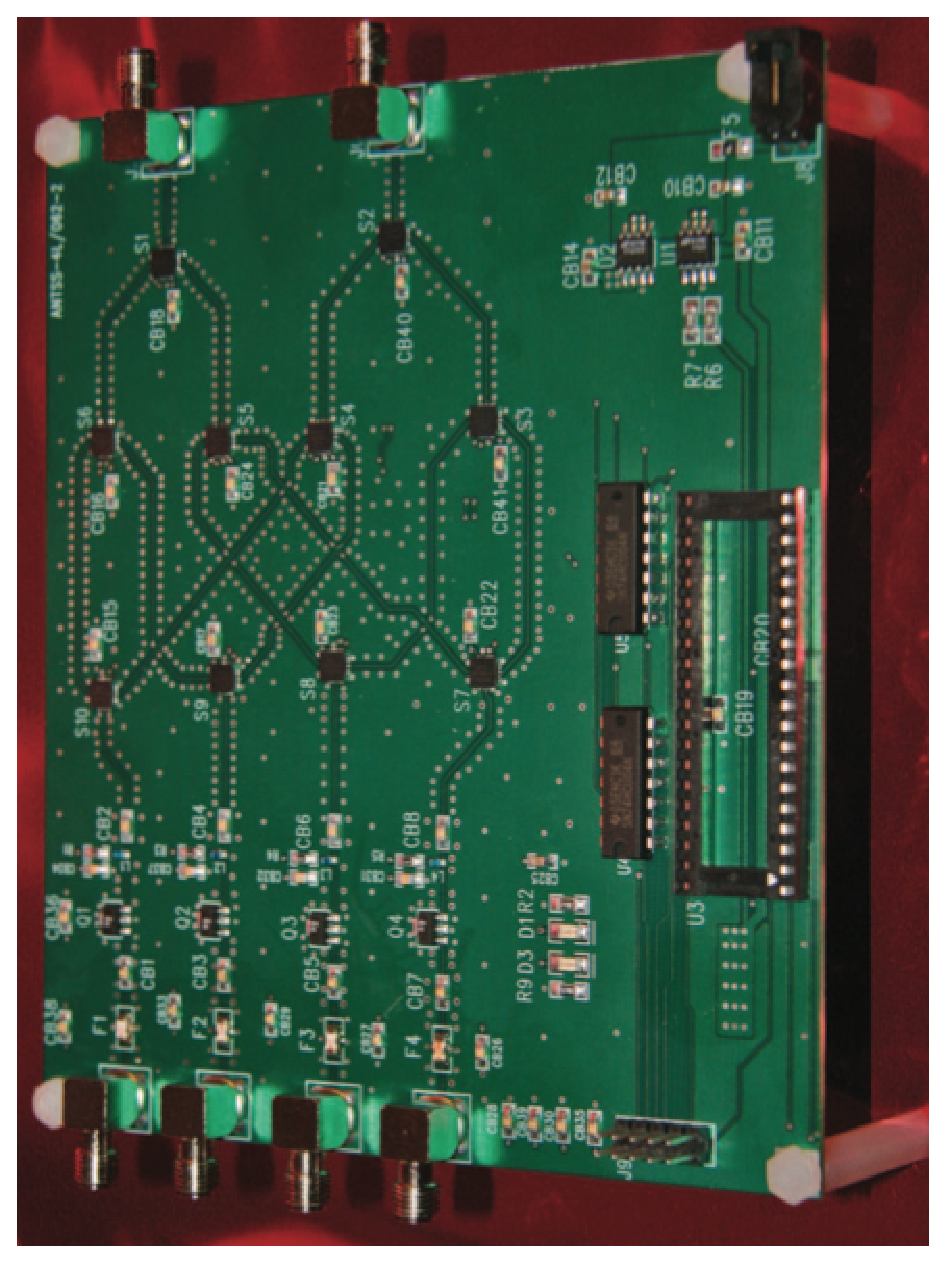
\includegraphics[scale=0.8]{ants_board.eps}
\caption{Single Antenna Subset Selection physical board}
\end{figure}

Unfortunately none of the control mechanisms in software have been created, therefore AntSS couldn't be fully tested and effectiveness determined.  This will be a reasonable avenue for future work.\\

\section{Summary}

This chapter discussed the implementation fall-backs and successes of the BLISS system.  The entire AS\textsuperscript{6} system was outlined and scrutinized for feasibility and operational performance.  Spectral Subtraction and Signal Separation were transitioned from original research goals to more manageable problems, with simplified solutions.  Overall it can be said that optimality and technical complexity were sacrificed in the end for realizability.  Many directions needed to be changed, especially in the Signal Separation block, and constraints needed to be tightened on the Spectral Subtraction block.  Although AntSS couldn't be realized a solid foundation exists for future work.\\ 




